



%\begin{figure*}[ht!]
%\centering
%\vspace{-3mm}
% \begin{subfigure}[b]{1.0\textwidth}
% \hspace{-10mm} 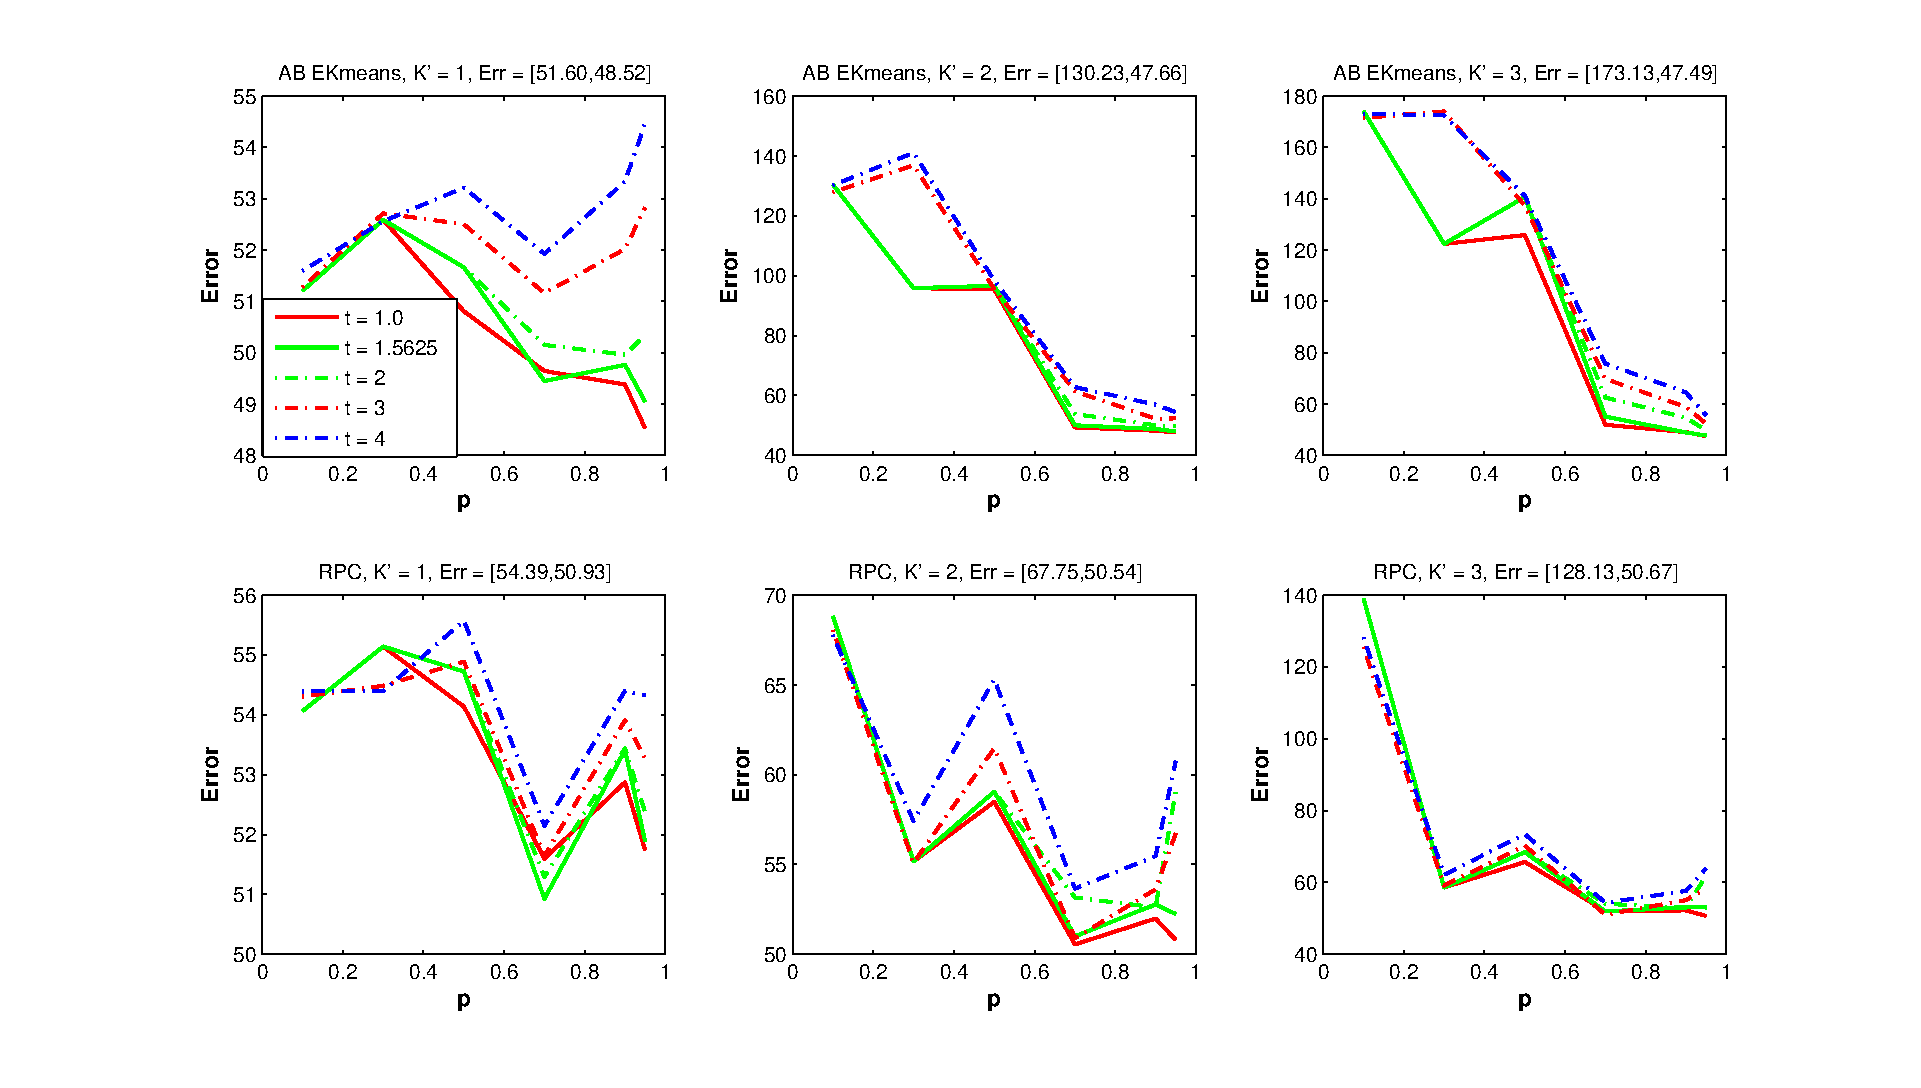
\includegraphics[width=1.0\textwidth,height=0.32\textwidth]{figGPR800HEva2.eps}
% \vspace{-4mm}
%   \hspace{-10mm}\caption{GPR-ODC (M=800) }
%\end{subfigure}
%\begin{subfigure}[b]{1.0\textwidth} 
% \hspace{-10mm}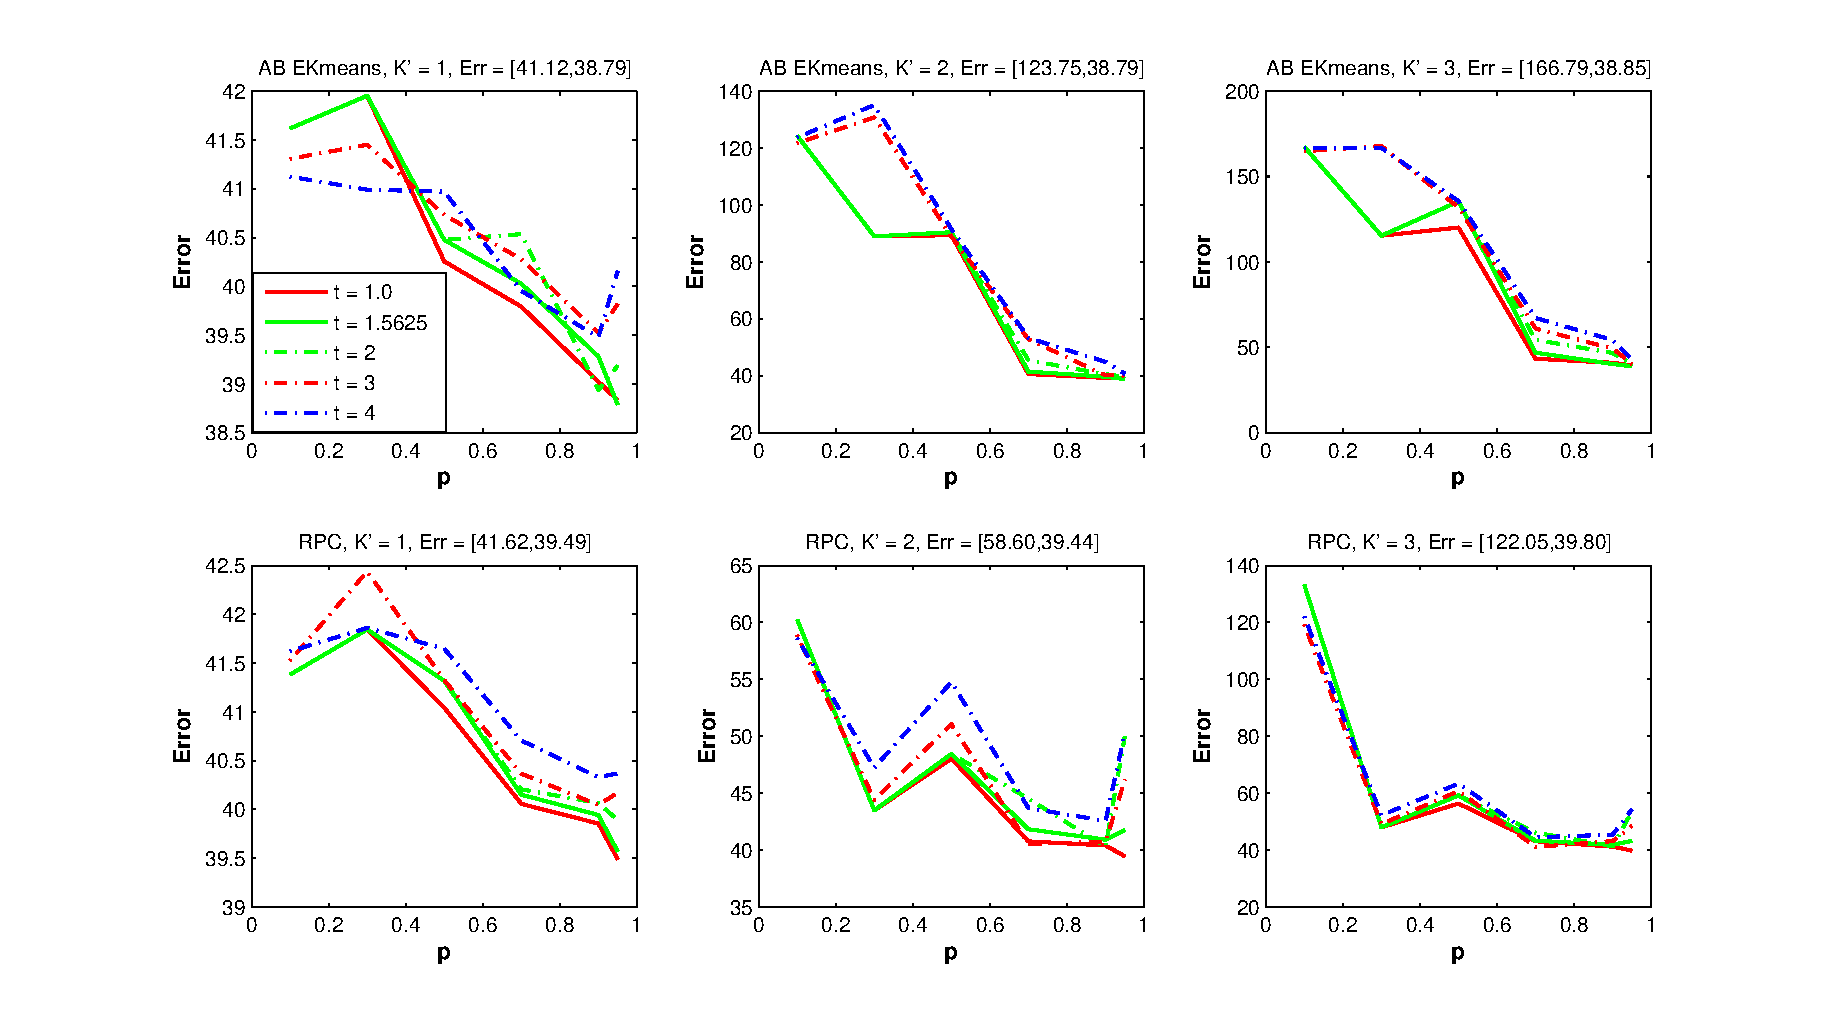
\includegraphics[width=1.0\textwidth,height=0.32\textwidth]{figTGP800HEva2.eps}
%  %\hspace{-15mm}
%  \vspace{-4mm}
%\caption{TGP-ODC (M=800)}
%\end{subfigure}
%  \vspace{-5mm}
%\caption{ODC framework Parameter Analysis of GPR and TGP  on Human Eva Dataset (best seen in color)}
%\label{fig:ODCAnalysis}
%\vspace{-5mm}
%\end{figure*}

\ignore{
In this section, we present our experimental evaluation. We start by evaluating the performance of the clustering algorithms, we proposed for the purpose of domain decomposition. Then, we discuss the performance of our ODC method on TGP and IWTGP only for space limit purpose. However, it is also applicable to GPR as presented. More results are attached in the supplementary materials}
\ignore{In this section, we present the experimental validation of our ODC-framework. We firstly present the datasets then the details of our experiments. }
%\subsection{Datasets, Features and Error Measures}




\textbf{Equal-Size Kmeans Step Experiment:}  We also tried another variant for Ekmeans that we call Iterative Minimum-Distance Assignments EKmeans (IMDA- Ekmeans).  Note that the algorithm presented earlier in the paper is denoted as Assign and Balance Kmeans (AB-Kmeans).  The IMDA- Ekmeans  algorithm works as follows. We initialize a pool of unassigned points $\tilde{X}  =  X$ and initialize all clusters as empty.  Given the means computed from the previous update steps, we compute the distances $d(\mathbf{x}_i,\mu_j)$ for all points/center pairs. We iteratively pick the minimum distance pair 
\[\small (\mathbf{x}_p,\mu_l)  : d(\mathbf{x}_p,\mu_l) \le d(\mathbf{x}_i,\mu_j)  \forall x_i \in \tilde{X} \text{and}  |C_l| < N/K \]
and assign point $x_p$ to cluster $l$. The point is then removed from the pool of unassigned points. if  $|C_l| = N/K$,  then it is marked as balanced and no longer considered. The process is repeated until the pool is empty; see Algorithm~\ref{alg:ddclusterALg2}. 

\begin{algorithm}[b!]
\KwIn{$\textbf{X} (N \times d_x ),{\{\boldsymbol{\mu}_i\}}_{i=1}^{K}$}
\KwOut{labels}
1- Create a matrix $\textbf{D} \in R^{N \times K}$, where $\textbf{D}[i,j]$ is the distance between the $i^{th}$ point to the $j^{th}$ cluster center.\\
2- Get the coordinate $(i_*,j_*)$ that maps the smallest distance in $\textbf{D}$.\\
3- Remove the $i_*^{th}$ row from matrix $\textbf{D}$ and mark it as assigned to the $j^{th}$ cluster\\
4- If the size of the cluster $j$ achieves the ideal size (i.e. ~ $n/K$), then remove the $j^{th}$ column from matrix $\textbf{D}$.\\
5- Go to step 2 if there is still unassigned points
\caption{Iterative Minimum-Distance Assignments (IMDA) k-means: Assignment Step}
\label{alg:ddclusterALg2}
\end{algorithm}


%\subsection{Iterative Minimum-Distance Assignments (IMDA) k-means EKmeans}



%\subsection{Comparison between IMDA and Assign and Balance (AB) EKmeans(presented in the paper) }
Table ~\ref{tab:clustering} presents the average cost over 10 runs of IMDA-Ekmeans and AB-Ekmeans algorithms. We initialize both the AB-Ekmeans and  IMDA-EKmeans algorithms by the cluster centers computed by running the standard k-means. As illustrated in table~\ref{tab:clustering}, the AB-Ekmeans  outperforms IMDA-Ekmeans in these experiments, which motivated us to utilize AB Ekmeans, which is presented in the paper, against  IMDA-Ekmeans under our ODC prediction framework.  Our interpretation for these results is because AB-Ekmeans initializes the assignment with an assignment that minimizes  the cost $J(C) = \min \sum_{j=1}^K \sum_{\mathbf{x_i}\in C_j} d(\mathbf{x_i}, \mu_j)$ given the cluster centers and then balance the clusters.  In all the following experiments, we uses AB-EKmeans due to its clear superior performance to IMDA-EKmeans. 


\begin{table}[htbp!]
  \centering
  \caption{$J(C)$ of AB-kmeans and  IMDA-kmeans on a dataset of 10,000 random 2D points, averaged over 10 runs}
    \label{tab:clustering}%
    \begin{tabular}{|c|c|c|c|}
    \hline
          & \textbf{K=5} & \textbf{K = 10} & \textbf{K=50} \\
              \hline
    \textbf{AB-kmeans} & 1077.3 & 540.241 & 105.505 \\
    \textbf{IMDA-kmeans} & 1290.6 & 657.446 & 122.006 \\
    \textbf{Error Reduction} & 16.53\% & 17.83\% & 13.52\% \\
    \bottomrule
    \end{tabular}% 
\end{table}%


\begin{figure}[th!]
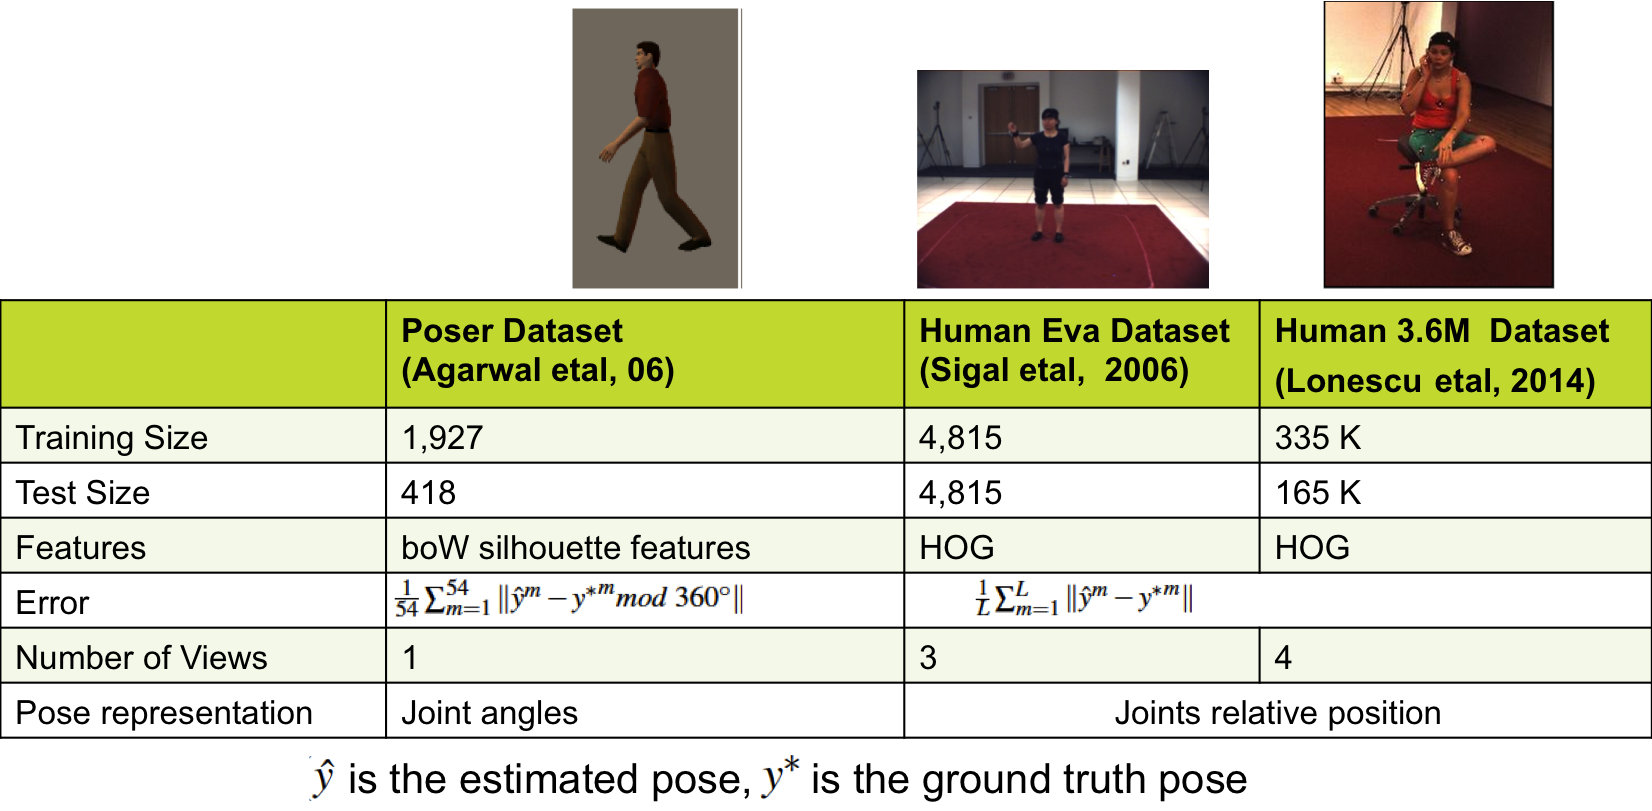
\includegraphics[width=0.5\textwidth]{datasets.png}
\caption{Datasets, Representations, and  Features}
\label{fig_datasets}
\end{figure}

\noindent \textbf{Datasets and Setup. } We evaluated our framework on three human pose estimation datasets, Poser, HumanEva, and Human3.6M; see Fig.~\ref{fig_datasets} for summary of setup and representation for each. \ignore{We here briefly describe the configuration, features, pose representation, and error measure for each dataset.} Poser dataset~\cite{Trig06} consists of 1927 training and 418 test images\ignore{, which are synthetically generated and tuned to unimodal predictions}. The image features, corresponding to bag-of-words representation with silhouette-based shape-context features. The error is measured by the root mean-square error (in degrees), averaged over all joints angles, and is given by: \small$Error(\hat{y}, y^*) = \frac{1}{54} \sum_{m=1}^{54} \| {\hat{y}}^m  - {y^*}^m mod$  $360^\circ \|$\normalsize , where $\hat{y} \in R^{54}$ is an estimated pose vector, and $y^* \in R^{54}$ is a true pose vector. HumanEva datset \cite{SigalBB10} contains synchronized multi-view video and Mocap data of 3 subjects performing multiple activities. We use  \ignore{histogram of oriented gradient (HOG)} HOG features~\cite{HOG05} (\small$\in R^{270}$\normalsize) proposed in \cite{Bo:2010}. We use training and validations subsets of HumanEva-I and only utilize data from 3 color cameras with a total of 9630 image-pose frames for each camera. This is consistent with experiments in \cite{Bo:2010} and \cite{Yamada:2012}. We use half of the data for training and half for testing. Human3.6M~\cite{human3m} is a dataset of millions of Human poses. We managed to evaluate our proposed ODC-framework on six Subjects (S1, S2, S6, S7, S8, S9) from it,  which is $\approx$ 0.5 million poses. We split them into  67\% training 33\% is testing. HOG features are extracted for 4 image-views for each  pose and concatenated into 3060-dim vector. Error for each pose, in both HEva (in $mm$) and Human 3.6 (in $cm$),  is measured as \ignore{average Euclidean distance:}\small$Error(\hat{y},y^*) = \frac{1}{L} \sum_{m=1}^{L} \|\hat{y}^m - {y^*}^m\|$\normalsize\ignore{, where $\hat{y}$ is an estimated pose vector, and $y^*$ is a true pose vector}. 


\begin{figure*}[t!]
\centering
\begin{tabular}{c}
{{{ 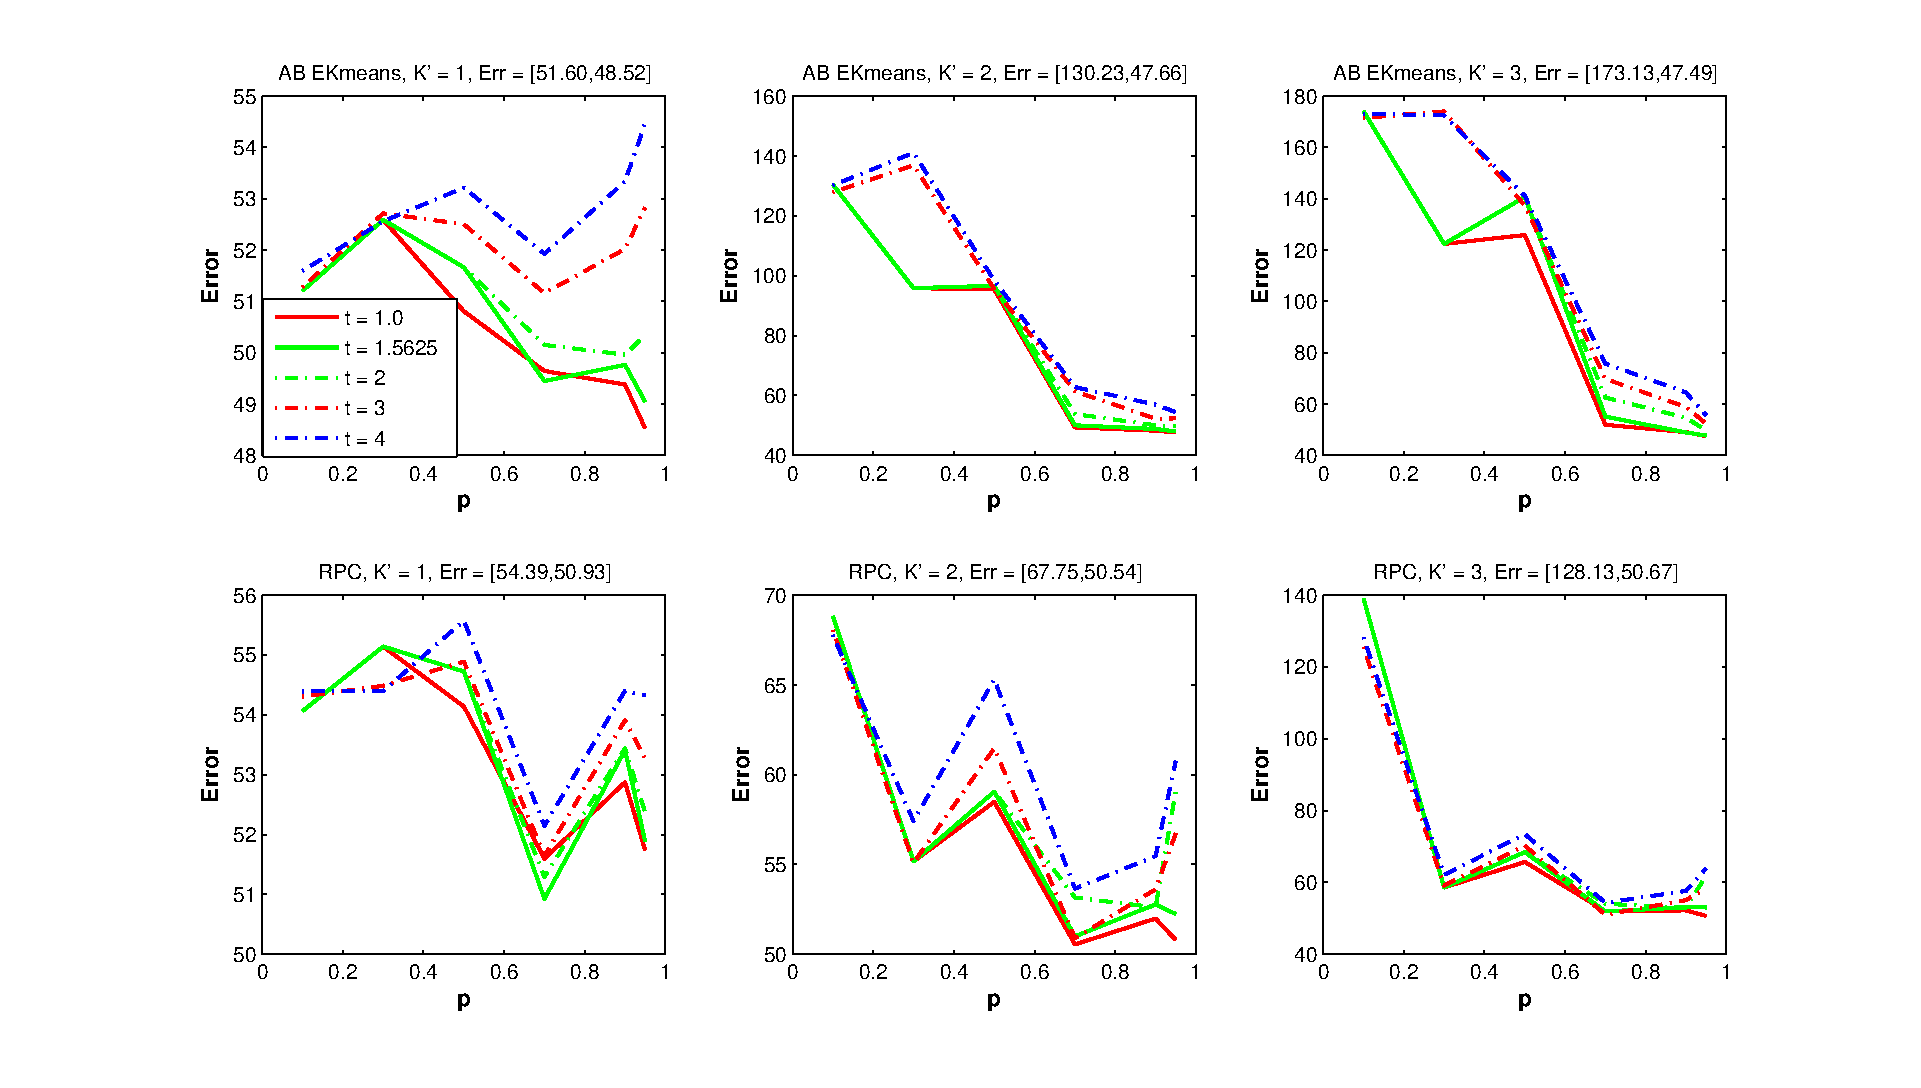
\includegraphics[width=1.0\textwidth,height=0.34\textwidth]{figGPR800HEva2.eps}}}}\\
 {(a) GPR-ODC (M=800) } \\
{{  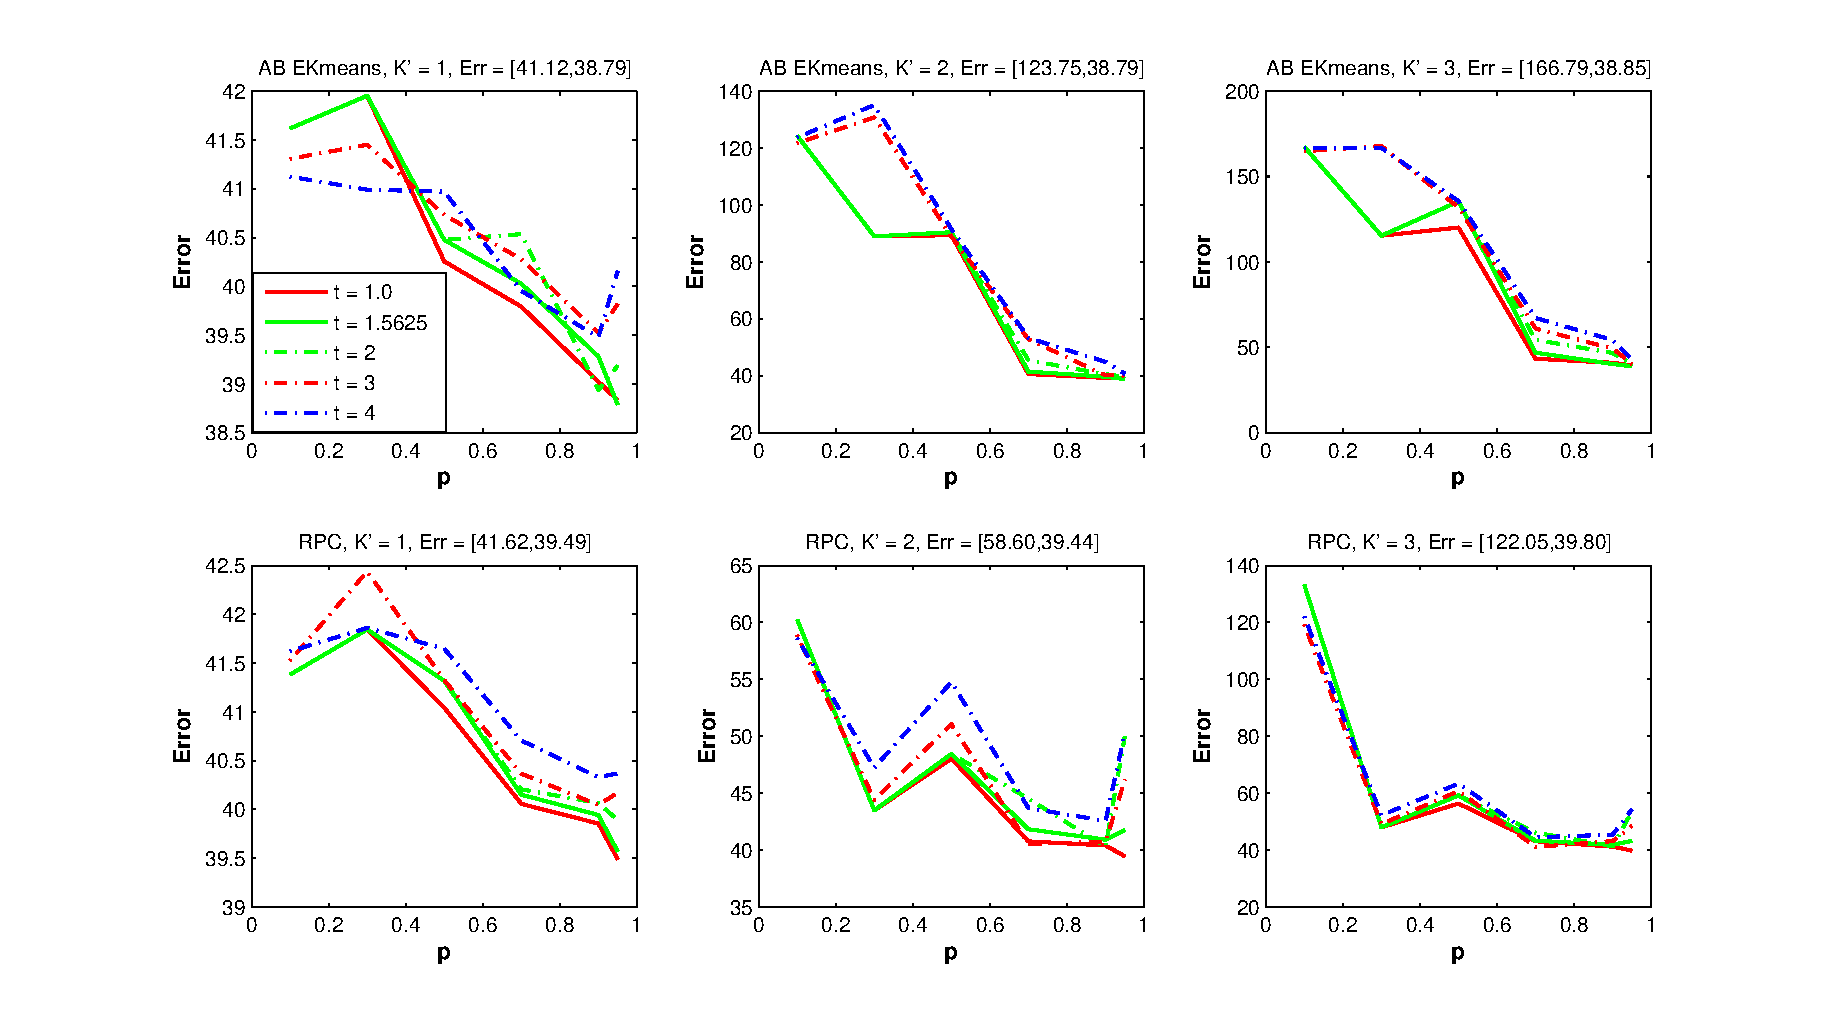
\includegraphics[width=1.0\textwidth,height=0.34\textwidth]{figTGP800HEva2.eps}}} \\
{ (b) TGP-ODC (M=800)} \\
\end{tabular}
\vspace{2mm}
\caption{ODC framework Parameter Analysis of GPR and TGP  on Human Eva Dataset}
\label{fig:ODCAnalysis}
%\label{fig:teaser}
\end{figure*}

\begin{table*}[t!]
  \centering
      %\vspace{4pt}
  \caption{Error \& Time on Poser and Human Eva datasets (Intel core-i7 2.6GHZ), M = 800}
    \scalebox{0.8}{
    \begin{tabular}{|l|l|lll|lll|}%ccc}
    \hline
          &   & \textbf{Poser} & \textbf{} &       & \textbf{HumanEva} &       &      \\% & \textbf{Human 3.6} &       &  \\
    \hline
         & & \textbf{Error (deg)} & \textbf{Training Time} & \textbf{Prediction Time} & \textbf{Error (mm) } & \textbf{Training Time} & \textbf{Prediction Time} \\%& \textbf{Error} & \textbf{Training Time} & \textbf{Prediction Time} \\
 \textbf{TGP}   & \textbf{NN ~\cite{Bo:2010}} & 5.43       &  -     &    188.99 sec   & \textbf{38.1}      &  -     & 6364 sec \\%       &       &       &  \\
%   & \textbf{Full} & \textbf{5.32 }     &    -  &   \textbf{27.5}  sec  &    \textbf{40.3 }  &  -   &  \textbf{1010} sec\\%       &       &       & 
  & \textbf{ODC ($p= 0.9, t=1, K'=1$)-Ekmeans} & \textbf{5.40 }     &      (3.7 +25.1 ) sec  &   \textbf{16.5}  sec  &    \textbf{38.9 }  &  (2001 + 45.4) sec    &  \textbf{298} sec\\%       &       &       &  \\
    & \textbf{ODC ($p= 0, t=1, K'=1$)-Ekmeans} &   7.60    &    (3.9 + 1.33) sec   &   14.8 sec  &    41.87   & (240 + 4.9 ) sec       &  257 sec \\%      &       &       &  \\
      &  \textbf{ODC ($p= 0.9, t=1, K'=1$)-RPC} & 5.60      &      (0.23 +41.6 ) sec  &   15.8 sec  &   39.9  &    ( 0.45 + 49.1) sec     & 277 sec\\%       &       &       &  \\
  &  \textbf{ODC ($p= 0, t=1, K'=1$)-RPC} &   7.70    &   (0.15 + 1.7) sec   &   13.89 sec  &  42.32    &  (0.19 + 5.2)      sec &  242 sec\\%      &       &       &  \\
      \hline
  \textbf{GPR}  & \textbf{NN} & 6.77      &   -    &  24 sec     &   54.8    &      - &    618  sec \\%&       &       &  \\
%   & \textbf{Full}  &  {6.10}      & -   &       \textbf{0.51}  sec & {59.62}  &   -  & \textbf{10.2} sec \\% 
   & \textbf{ODC ($p= 0.9, t=1 , K'=1$)-Ekmeans} &  \textbf{6.27}      &  (3.7 +11.1 ) sec  &       \textbf{0.56}  sec & \textbf{49.3}  &   (2001 + 42.85)sec & \textbf{79} sec \\%       &       &       &  \\
   & \textbf{ODC($p= 0.0, t=1 , K'=1$)-Ekmeans} & 7.54      &   ( 3.9 + 1.38 sec) &    0.35 sec   & 49.6  &  (240 + 6.4) sec  &  48 sec\\%      &       &       &  \\
  & \textbf{ODC ($p= 0.9, t=1 , K'=1$)-RPC} &  6.45      &  (0.23 +17.3 ) sec  &       0.52  sec & 52.8  & (0.49 + 46.06) sec     &  64 sec\\%       &       &       &  \\
    & \textbf{ODC ($p= 0.0, t=1 , K'=1$)-RPC  = ~\cite{Chalupka:2013}} &   7.46    &   (0.15 + 1.5) sec &    0.27 sec   & 54.6  &  (0.26 + 4.6 ) sec & 44 sec\\%      &       &       &  \\
    & \textbf{FIC ~\cite{fic06}} &   7.63   &   (- + 20.63)   &    0.3106     &   68.36   &  -     & 102  sec\\%      &       &       &  \\
    \hline
    \end{tabular}}%
  \label{tab:tblRes}%
  \vspace{-5mm}
\end{table*}%

%\subsection{Experiments}
%\def\arraystretch{0.8}
There are four control parameters in our ODC framework: $M$, $p$, $t$, and $K'$.\ignore{We started by performing inherent analysis of these parameters.} Figure~\ref{fig:ODCAnalysis}  shows our parameter analysis with different values of $p$, $t$ and $K'$ on HumanEva dataset  for GPR and TGP as local regression machines, where $M=800$.  Each sub-figure consists of six plots in two rows. The first row indicates the results using AB-Ekmeans clustering scheme, while the second row shows the results for RPC clustering scheme. Each row has three plots, one for $K'=1$, $2$, and $3$ respectively. 
\ignore{\begin{figure}[t!]
\centering
\begin{tabular}{c}
\bmvaHangBox{{{ 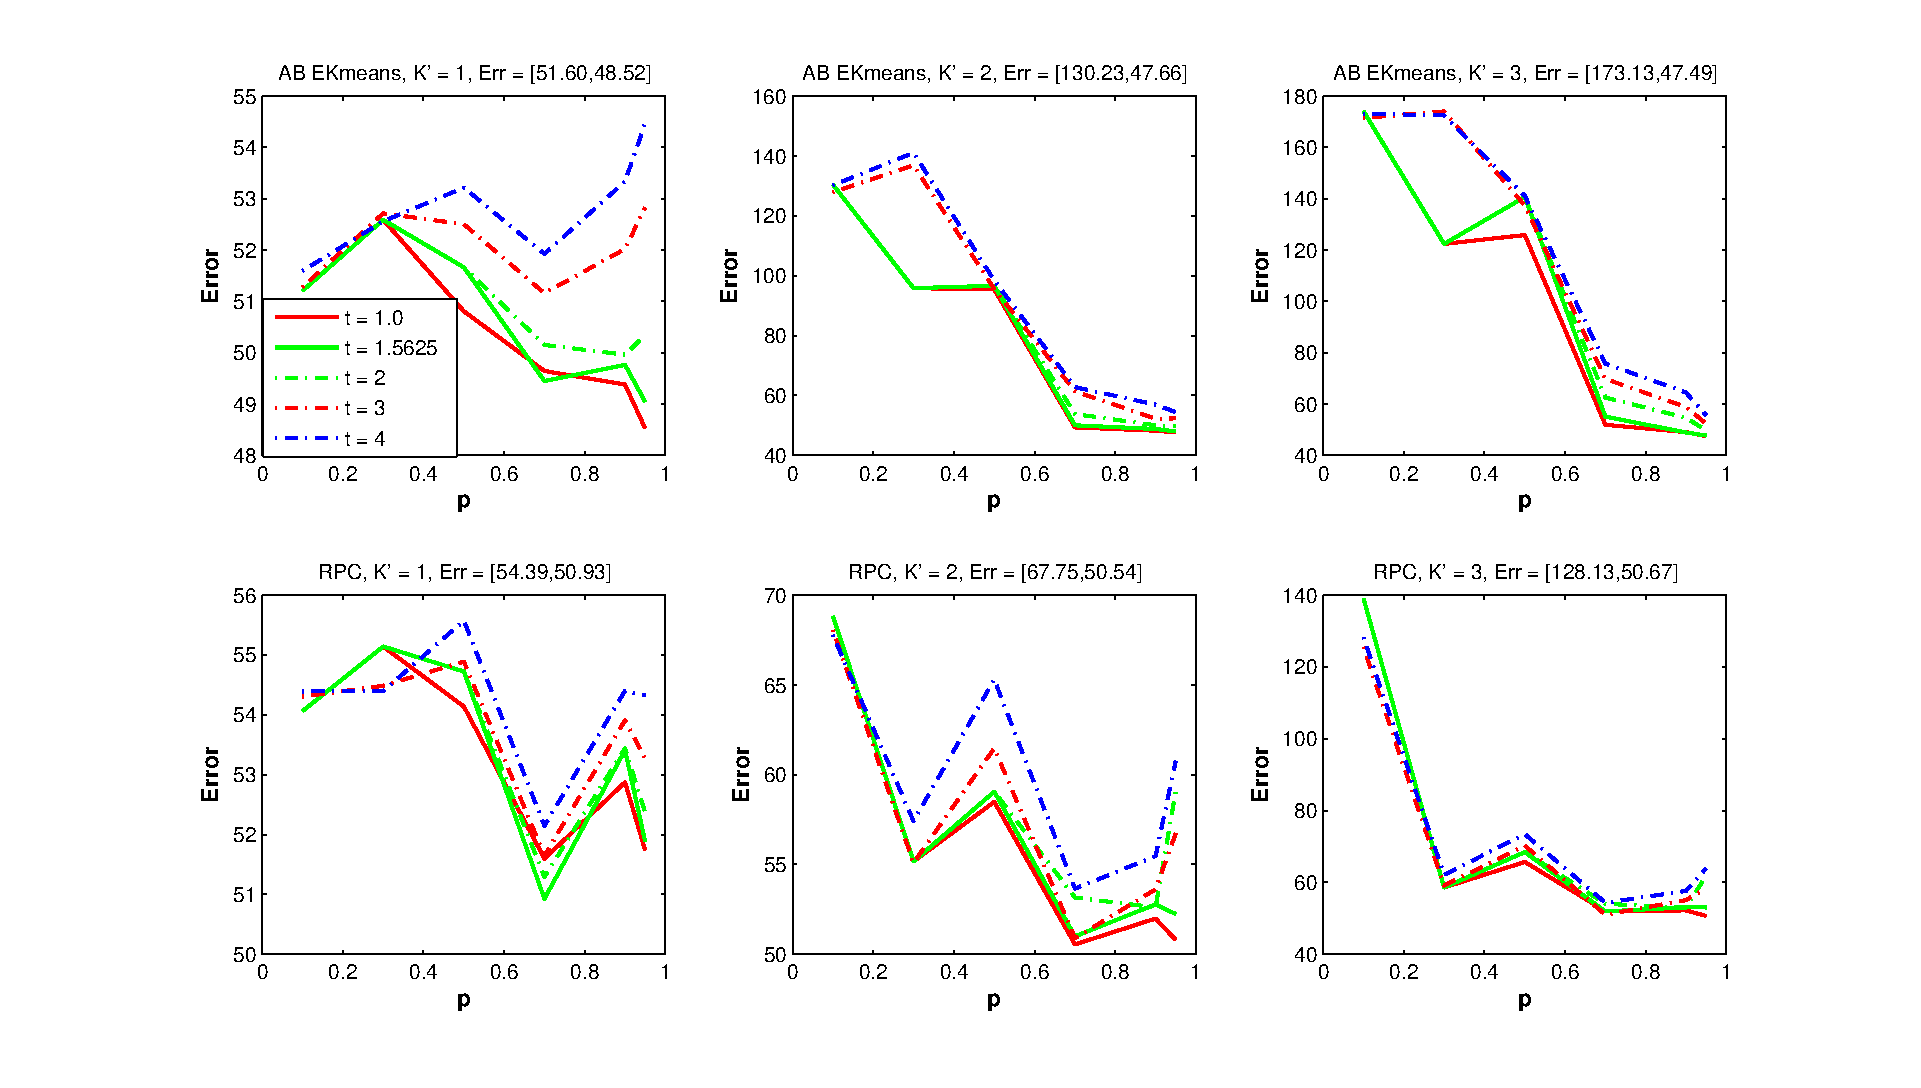
\includegraphics[width=1.0\textwidth,height=0.34\textwidth]{figGPR800HEva2.eps}}}} \\
\vspace{-7mm}
 {\tiny(a) GPR-ODC (M=800) } \\
\bmvaHangBox{{  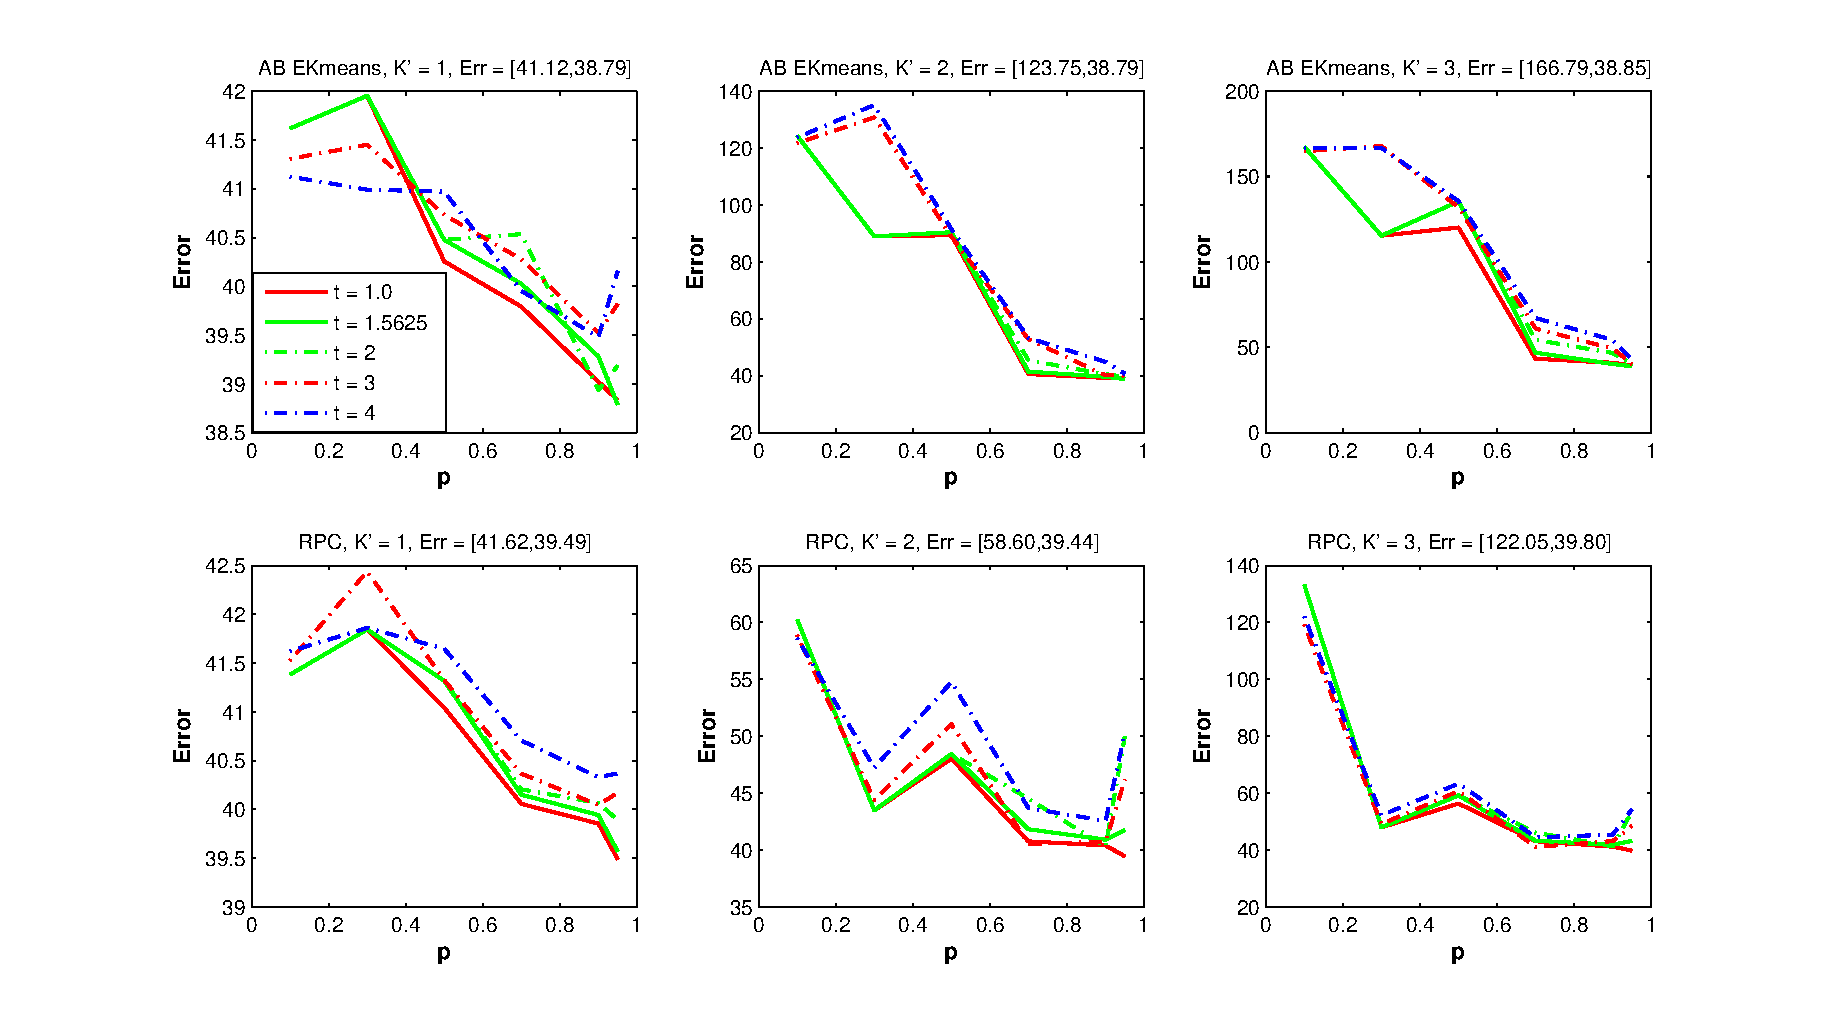
\includegraphics[width=0.\textwidth,height=0.34\textwidth]{figTGP800HEva2.eps}}}\\
 \vspace{-7mm}
{ \tiny (b) TGP-ODC (M=800)} \\
\ignore{\bmvaHangBox{{  \includegraphics[width=1.0\textwidth,height=0.34\textwidth]{figTGP400HEva.eps}}}\\
(c) TGP-ODC (M=400) \\}
\end{tabular}
\caption{ODC framework Parameter Analysis of GPR and TGP  on Human Eva Dataset (seen in color)}
\label{fig:ODCAnalysis}
\vspace{-15mm}
\end{figure}}
\begin{comment}
\begin{figure}[h!]
\centering
\begin{tabular}{cc}
 {\footnotesize (a) GPR-ODC (M=800) } &
\bmvaHangBox{{{     \includegraphics[width=1.0\textwidth,height=0.34\textwidth]{figGPR800HEva.eps}}}} \\
 { \footnotesize (b) TGP-ODC (M=800)}  &
\bmvaHangBox{{  \includegraphics[width=1.0\textwidth,height=0.34\textwidth]{figTGP800HEva.eps}}}\\
\ignore{\bmvaHangBox{{  \includegraphics[width=1.0\textwidth,height=0.34\textwidth]{figTGP400HEva.eps}}}\\
(c) TGP-ODC (M=400) \\}
\end{tabular}
\vspace{2mm}
\caption{Overlapping Domain Cover Parameter Analysis of GPR and TGP  on Human Eva Dataset (best seen in color)}
\label{fig:ODCAnalysis}
\vspace{-15mm}
%\label{fig:teaser}
\end{figure}
\end{comment}
Each plot shows the error of different $t$ against $p$ from 0 to 0.95; i.e., it shows how the overlap affects the performance for different values of $t$. Each plot shows, on its top caption, the minimum and the maximum overlap regression errors where $t \to 1$. Looking at these plots, there are a number of observations:

\noindent\textbf{(1)} As $t \to 1$ (the solid red line), the behavior of the error tends to reduce as $p$ increases, i.e., the overlap.

\noindent\textbf{(2)} Comparing different $K'$, the behavior of the error indicates that combining multiple predictions (i.e., $K'=2$ and $K'=3$), gives poor performance, compared with  $K'=1$,  when the overlap is small. However, all of them, $K'=1$, $2$, and  $3$, performs well as  $p \to 1$; see column 2 and 3 in Fig.~\ref{fig:ODCAnalysis} and Fig.~\ref{fig_K_all}.  This indicates consistent prediction of neighboring subdomains as $p$ increases; see also Fig.~\ref{fig_K_each} for side by side comparison of different $K'$. The main reason behind this behavior is  that as $p$ increases, the local models of the  neighboring subdomains normally share more training points on their boundaries, which is reflected as shared constraints during the training of these models making them more consistent on prediction. 

\noindent\textbf{(3)} Comparing the first row to the second row in each subfigure, it is not hard to see that our AB-Ekmeans partitioning scheme consistently \ignore{ends up with better error rates compared with} outperforms RPC \cite{Chalupka:2013}, \eg the error in cases of  GPR (M=800) is  47.48mm for AB-EKmeans and 50.66mm for RPC, TGP (M=800) is  38.8mm for AB-EKmeans and 39.8mm for RPC. This problem is even more severe when using smaller $M$, \eg the error in case of \ignore{ GPR (M=400) is 45.20mm for EKmeans and 50.56mm for RPC, } TGP (M=400) is 39.5mm for EKmeans and 47.5mm for RPC; see a detailed plot for M=400 in Fig.~\ref{fig:ODCAnalysis400}.  We noticed sigficant drop in the performance as M decreases. For instance when $M=200$, The error for TGP best performance increased to 43.88mm instead of 38mm for $M=800$.  

\noindent\textbf{(4)} TGP gives better prediction than GPR (i.e., 38mm using TGP compared with 47mm using GPR). 

\noindent\textbf{(5)} As $M$ increases, the prediction error decreases. For instance, when $M=200$, The error for TGP best performance increased to 43.88mm instead of 38.9mm for $M=800$. We found these observation to be also consistent on Poser dataset. 
\begin{figure*}[t!]
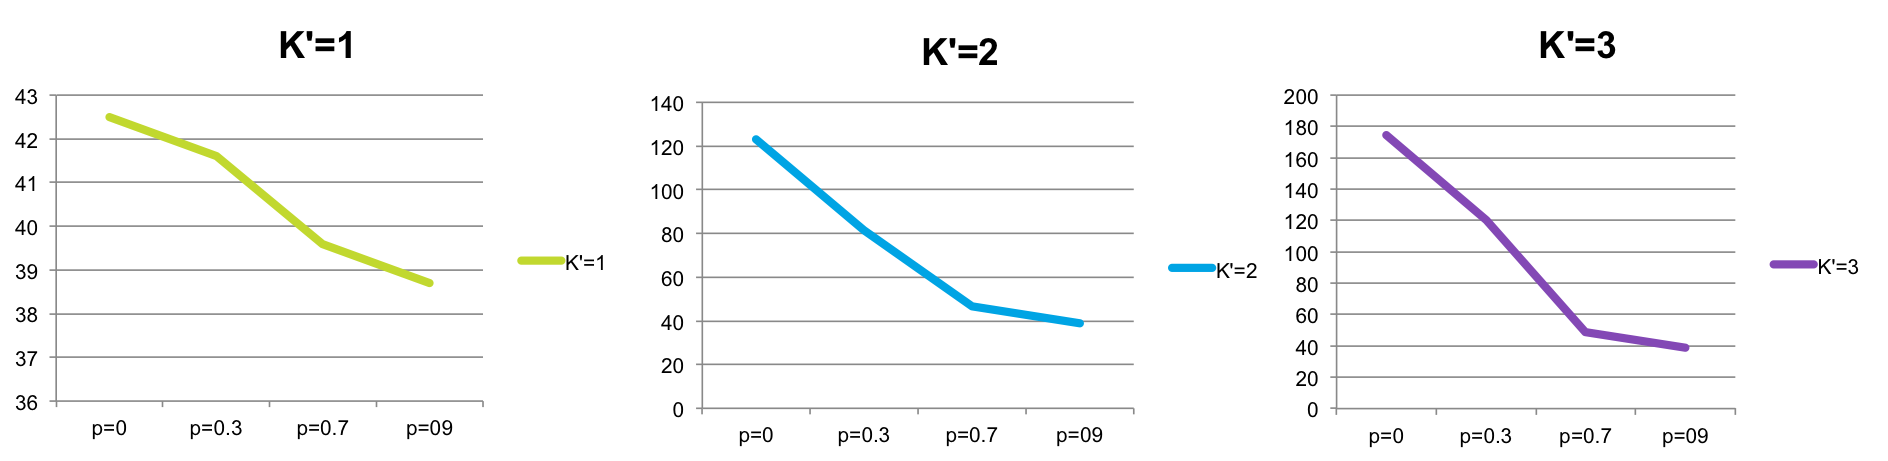
\includegraphics[width=1.0\textwidth]{HEVa_TGP_Kp_each.png}
\caption{HumanEva TGP different K' as overlap increase, ,  M=800}
\label{fig_K_each}
\end{figure*}

\begin{figure}[t!]
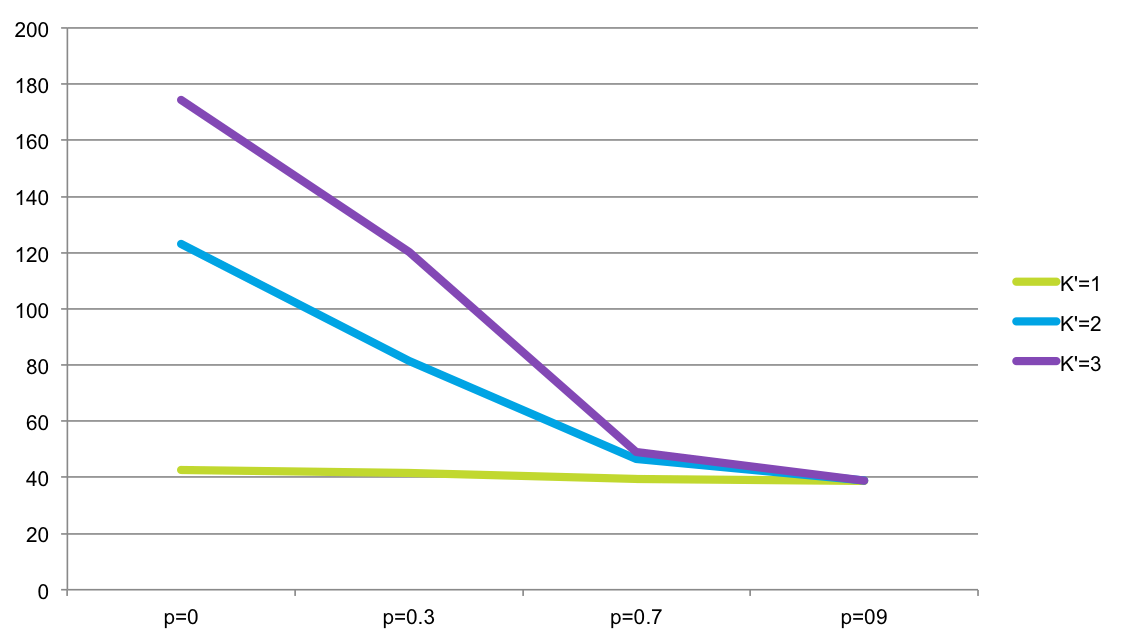
\includegraphics[width=0.5\textwidth]{HEVa_TGP_Kp_all.png}
\caption{Increasing K' significantly heart the performance for small overlap (Human Eva TGP,  M=800)}
\label{fig_K_all}
 % \label{fig:SpeedUp}
\end{figure}

\begin{figure*}[h!]
\centering
\begin{subfigure}[b]{1.0\textwidth}
 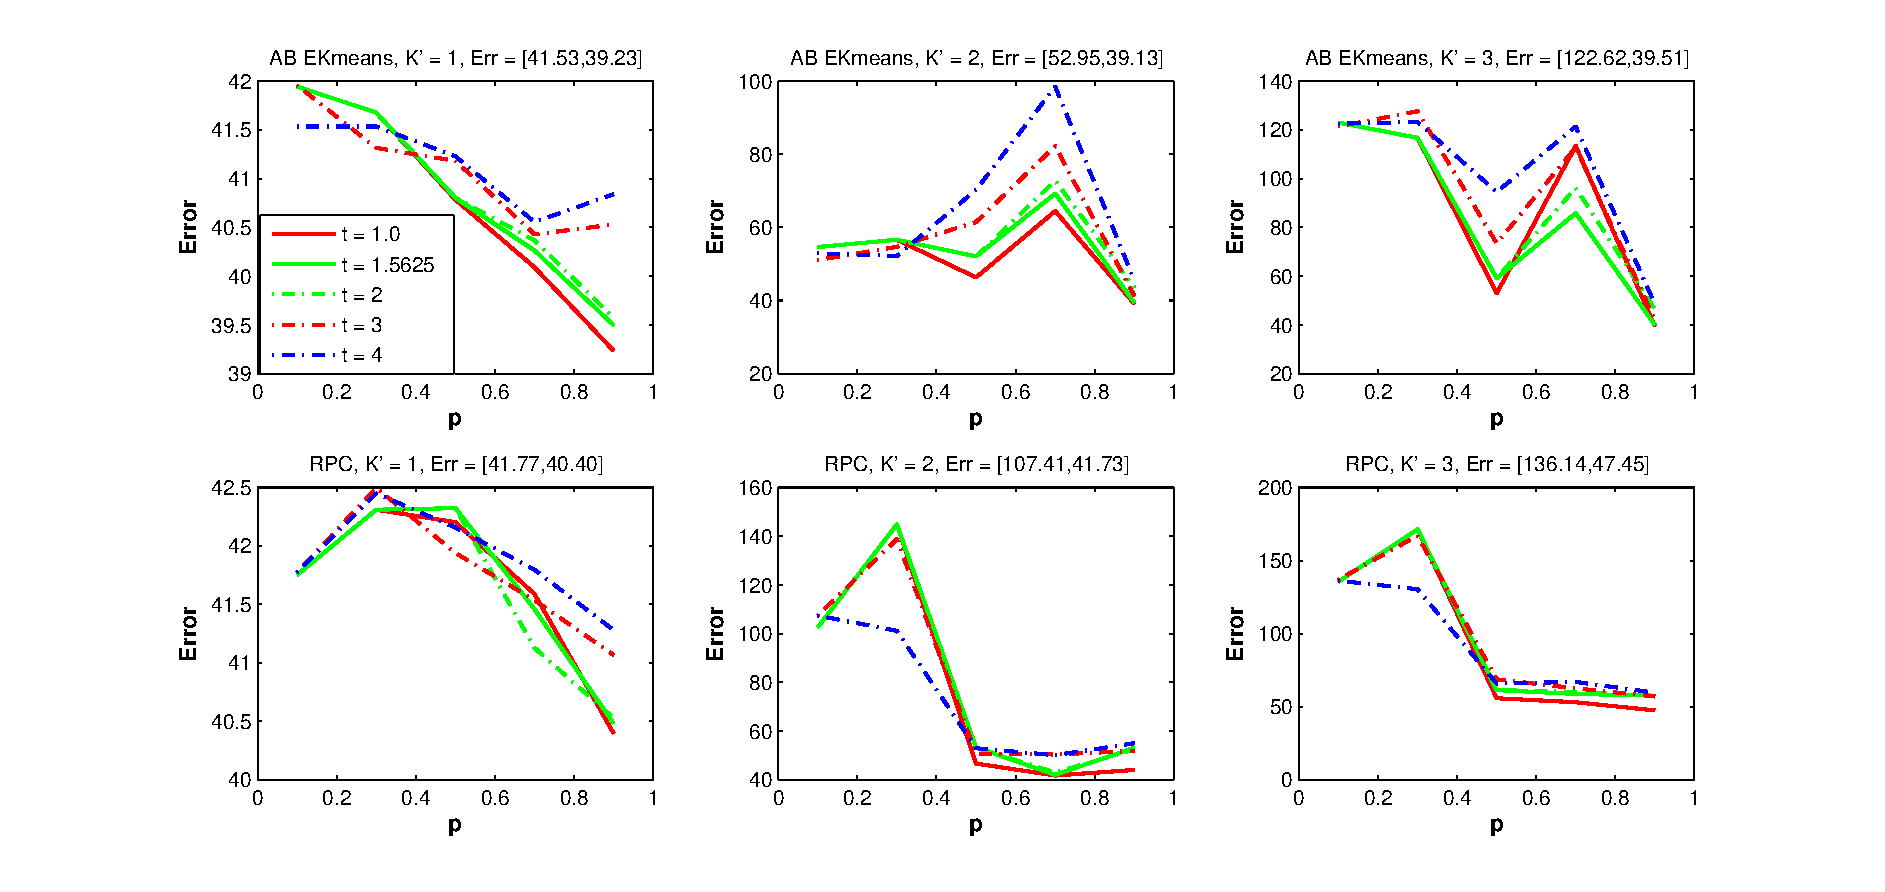
\includegraphics[width=1.0\textwidth,height=0.34\textwidth]{figTGP400HEva2.eps}
  \caption{TGP-ODC (M=400)}
\end{subfigure}
\begin{subfigure}[b]{1.0\textwidth} 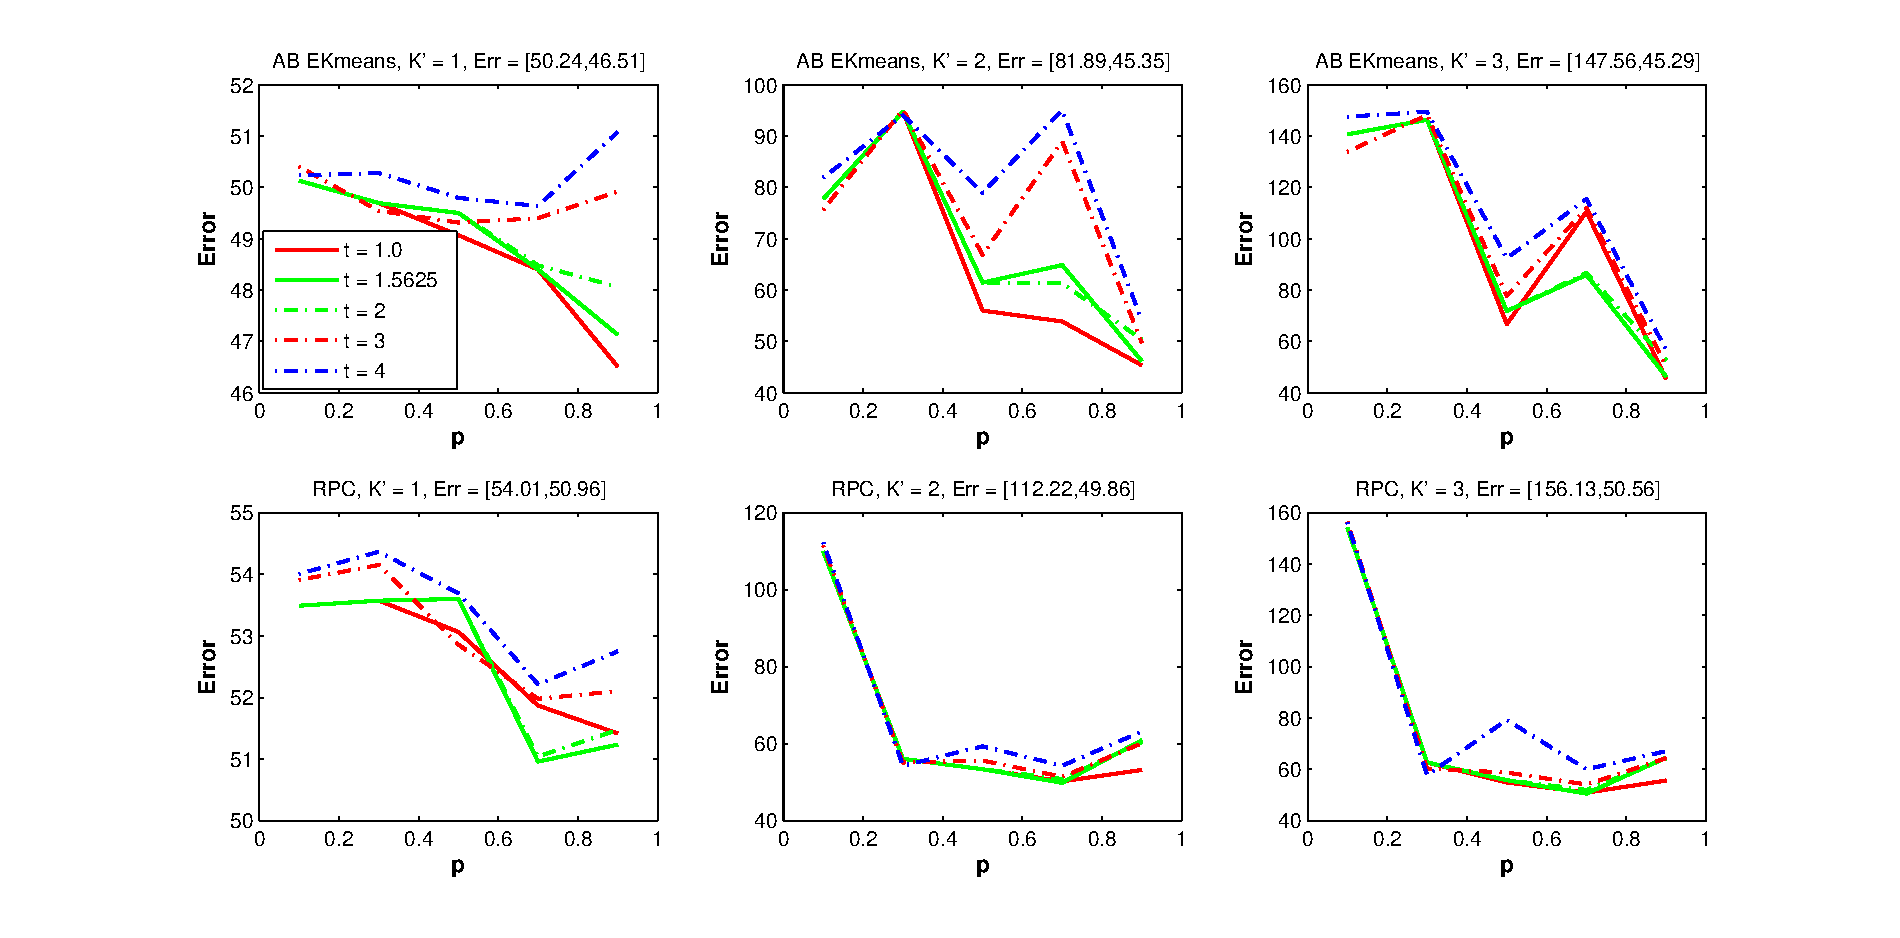
\includegraphics[width=1.0\textwidth,height=0.34\textwidth]{figGPR400HEva2.eps}
\caption{GPR-ODC (M=400)}
\end{subfigure}
\caption{Overlapping Domain Cover Parameter Analysis of GPR and TGP  on Human Eva Dataset (best seen in color) (M=400)}
\label{fig:ODCAnalysis400}
%\label{fig:teaser}
\end{figure*}


This analysis helped us conclude recommending choosing  $t$ close to $1$, big overlap ($p$ closer to 1), and $K'=1$ is sufficient for accurate prediction. \ignore{
\begin{wrapfigure}{r}{0.3\textwidth}
\centering
  \vspace{-10pt}
  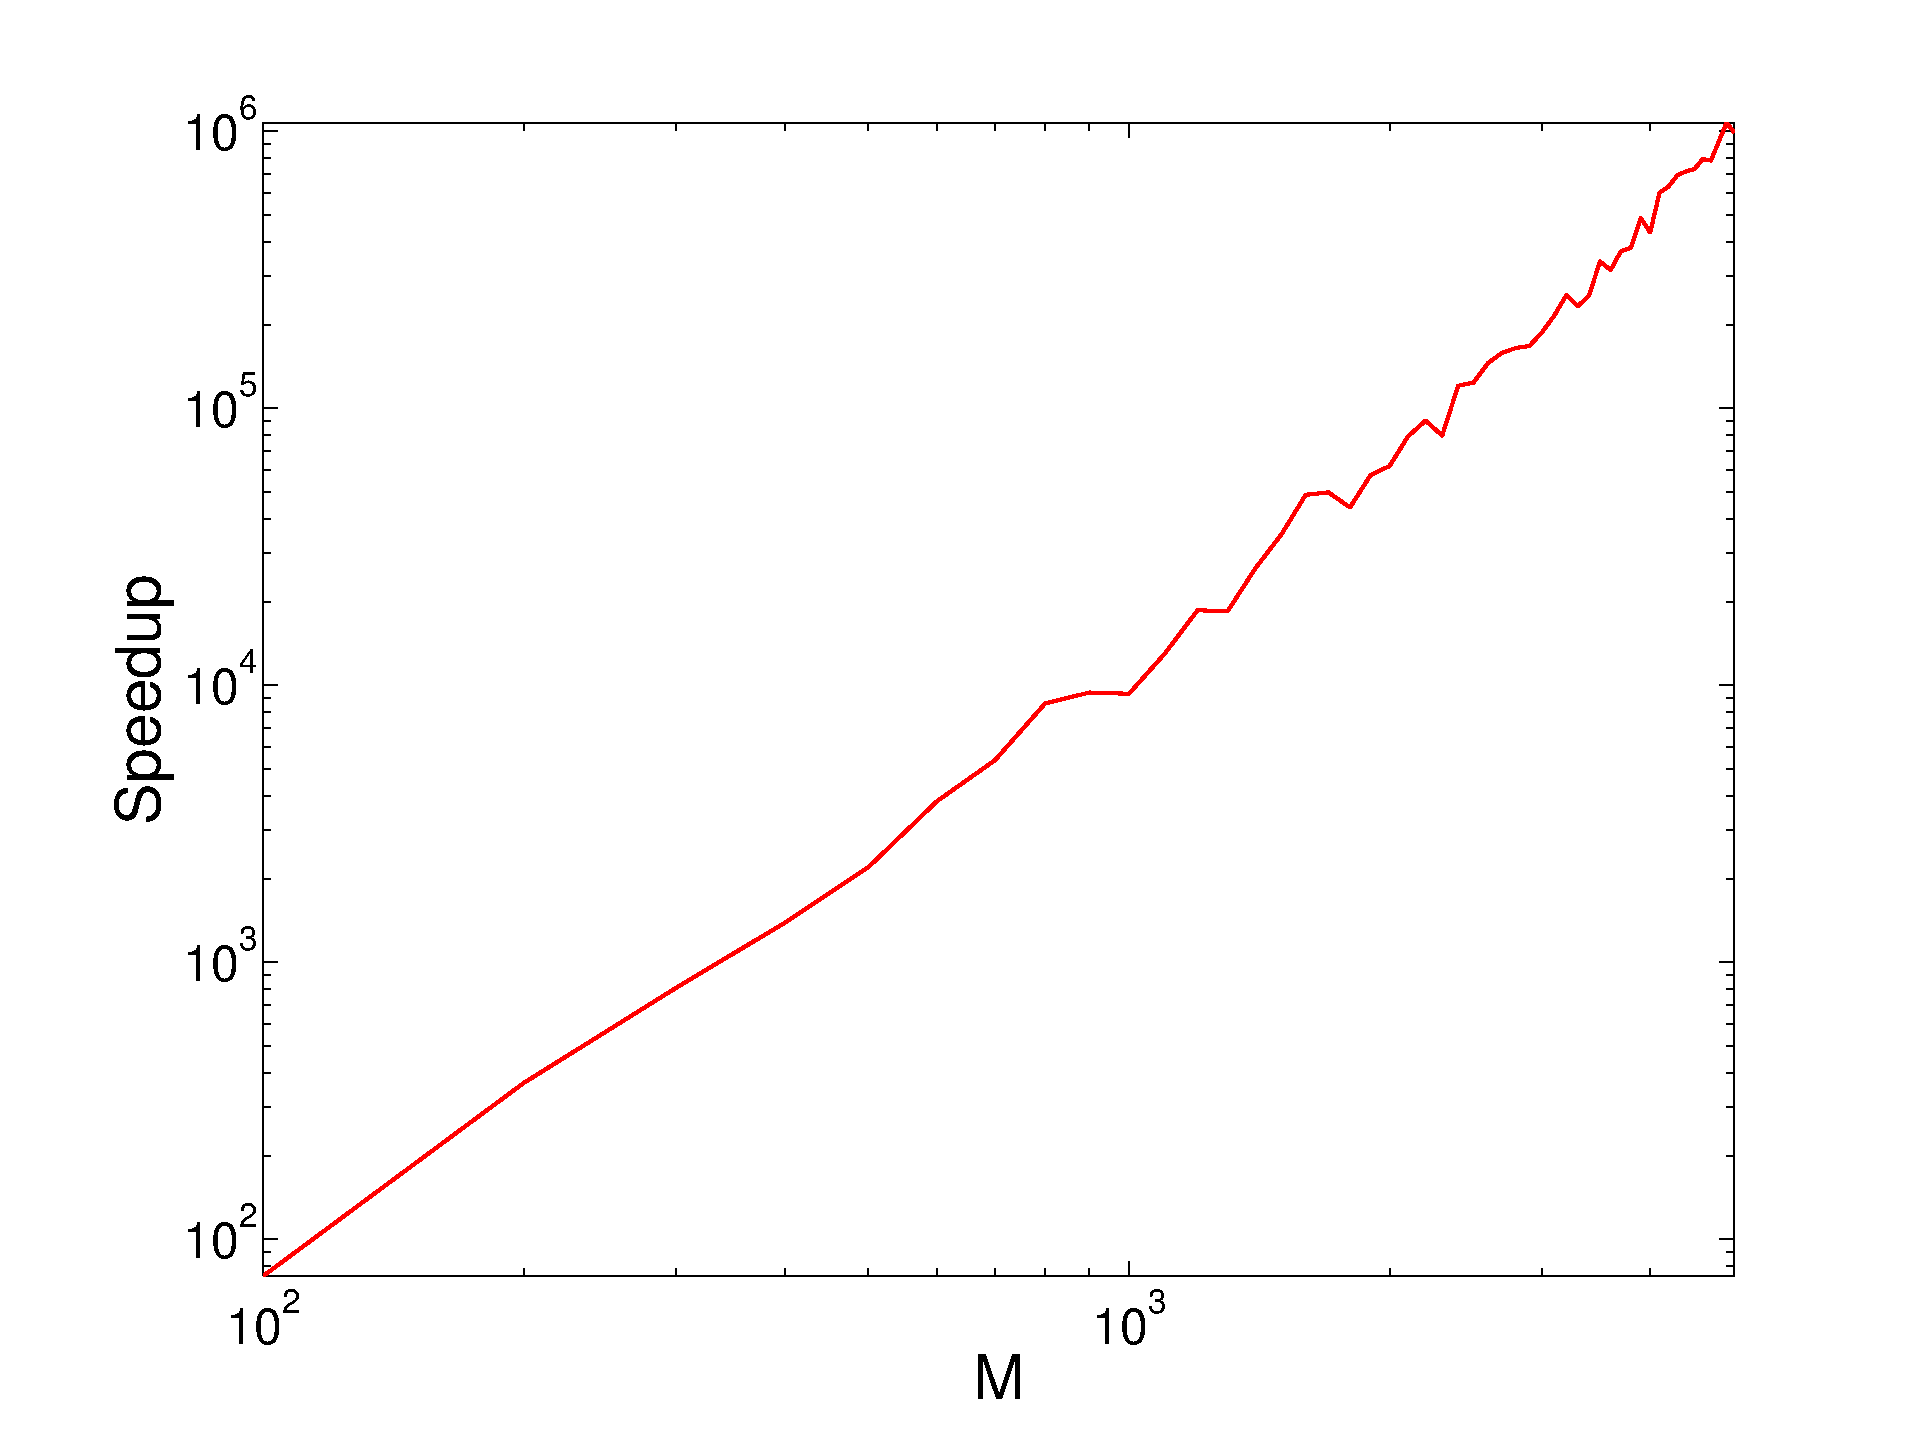
\includegraphics[width=0.35\textwidth]{figMInvSpeedUp.eps}
  \vspace{-10pt}
  \caption{Matrix Inverse Precomputation Speedup of ODC framework prediction as $M$ increases (log-log scale)}
  \label{fig:SpeedUp}
\end{wrapfigure}}





%\begin{wrapfigure}{r}{6.5cm}\vspace{-6mm}
%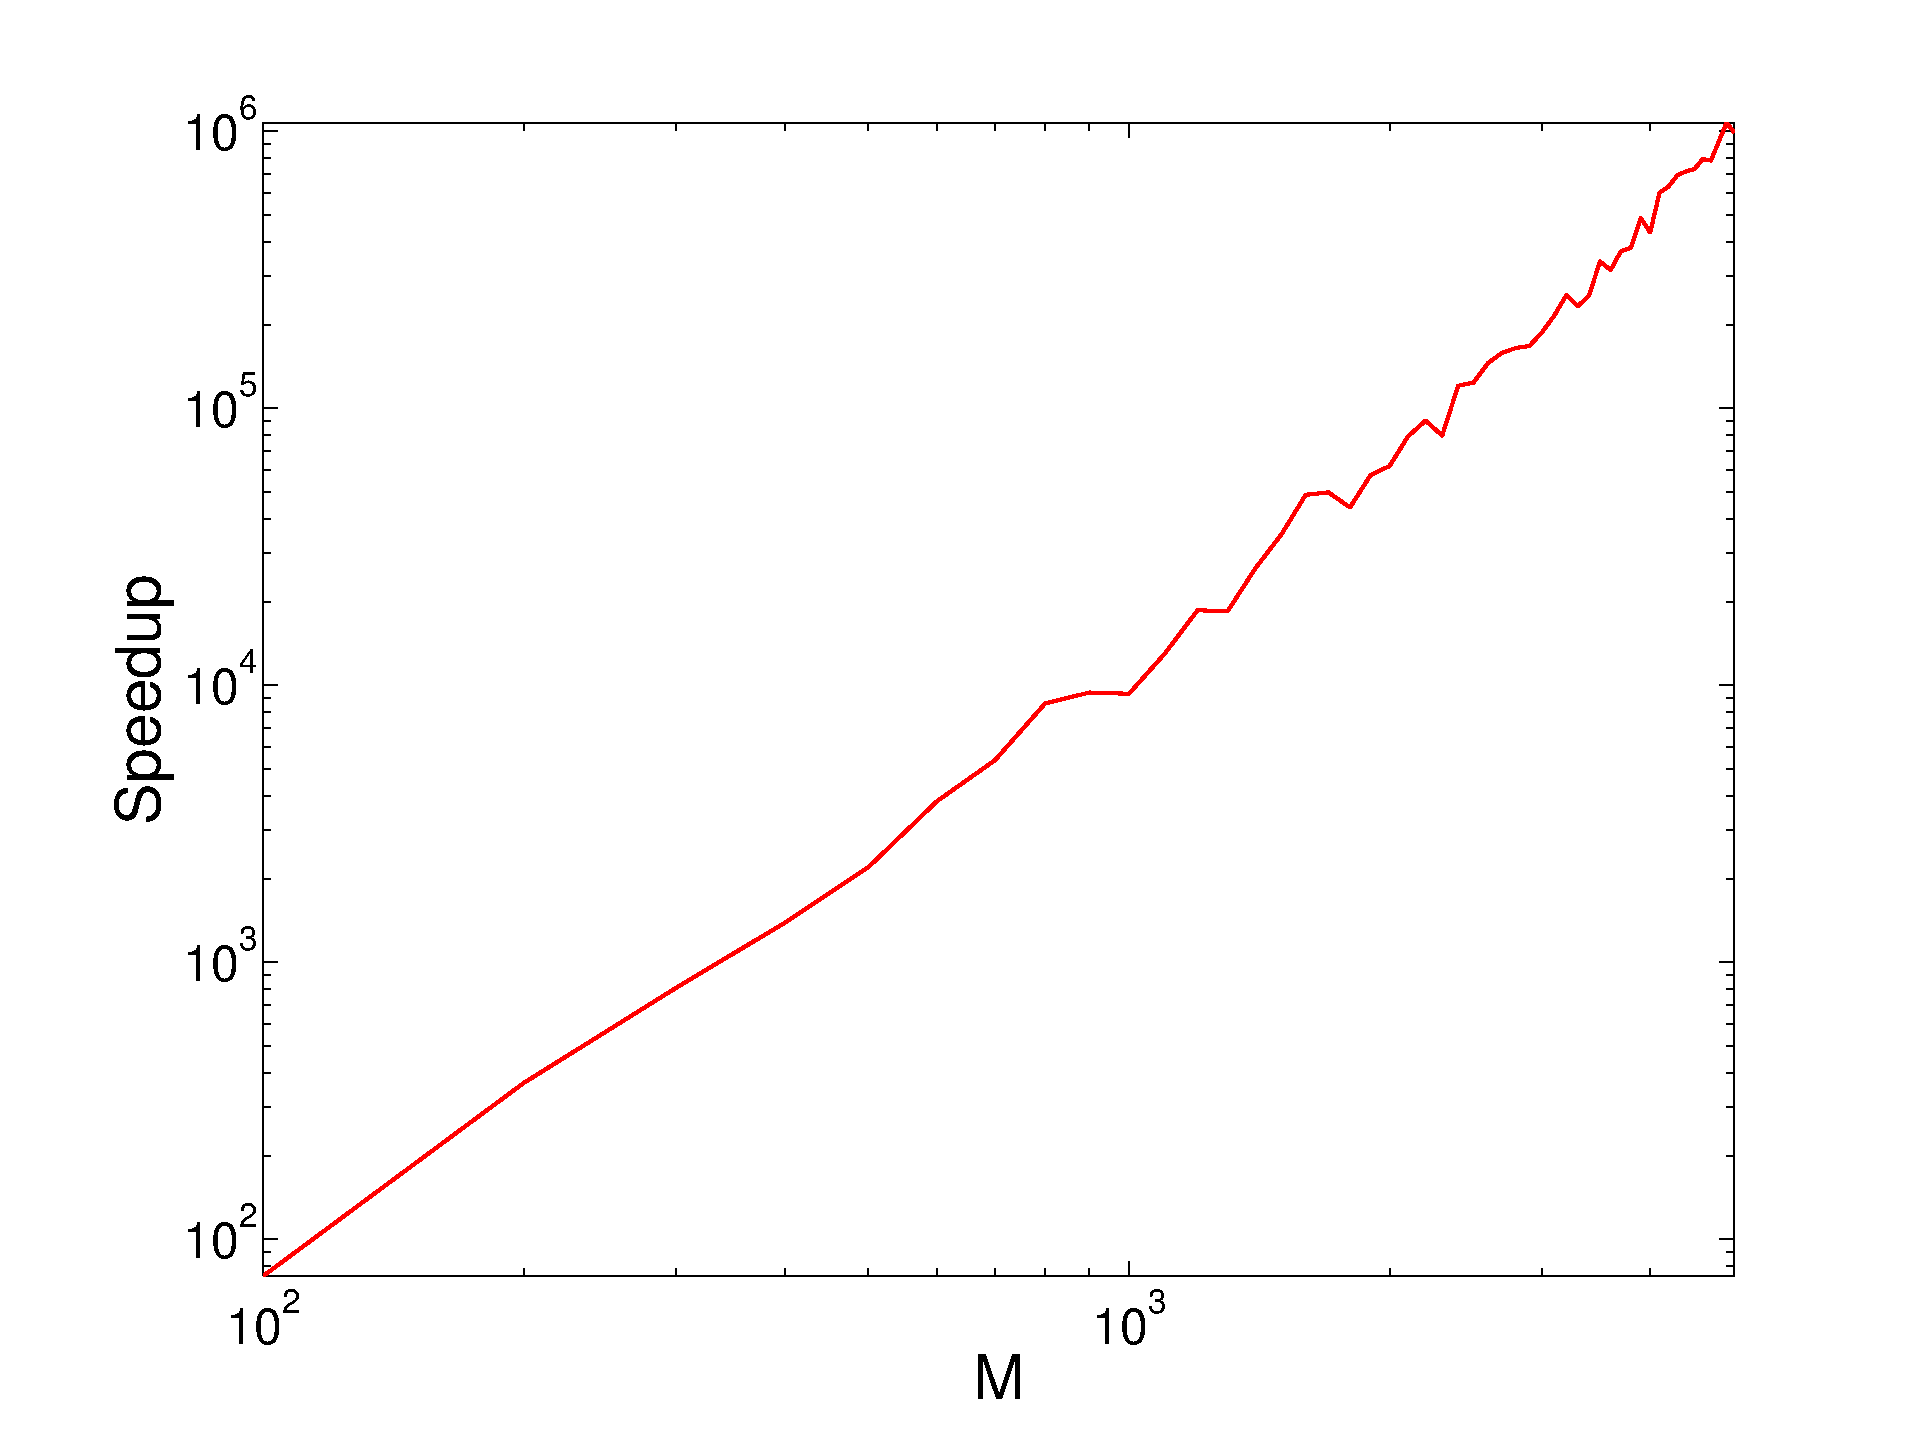
\includegraphics[width=6.5cm]{figMInvSpeedUp.eps}
%\caption{Matrix Inverse Precomputation Speedup of ODC framework prediction as $M$ increases (log-log scale)}\vspace{-4mm}\label{fig:SpeedUp}\end{wrapfigure}
\begin{figure}[h!]
\centering
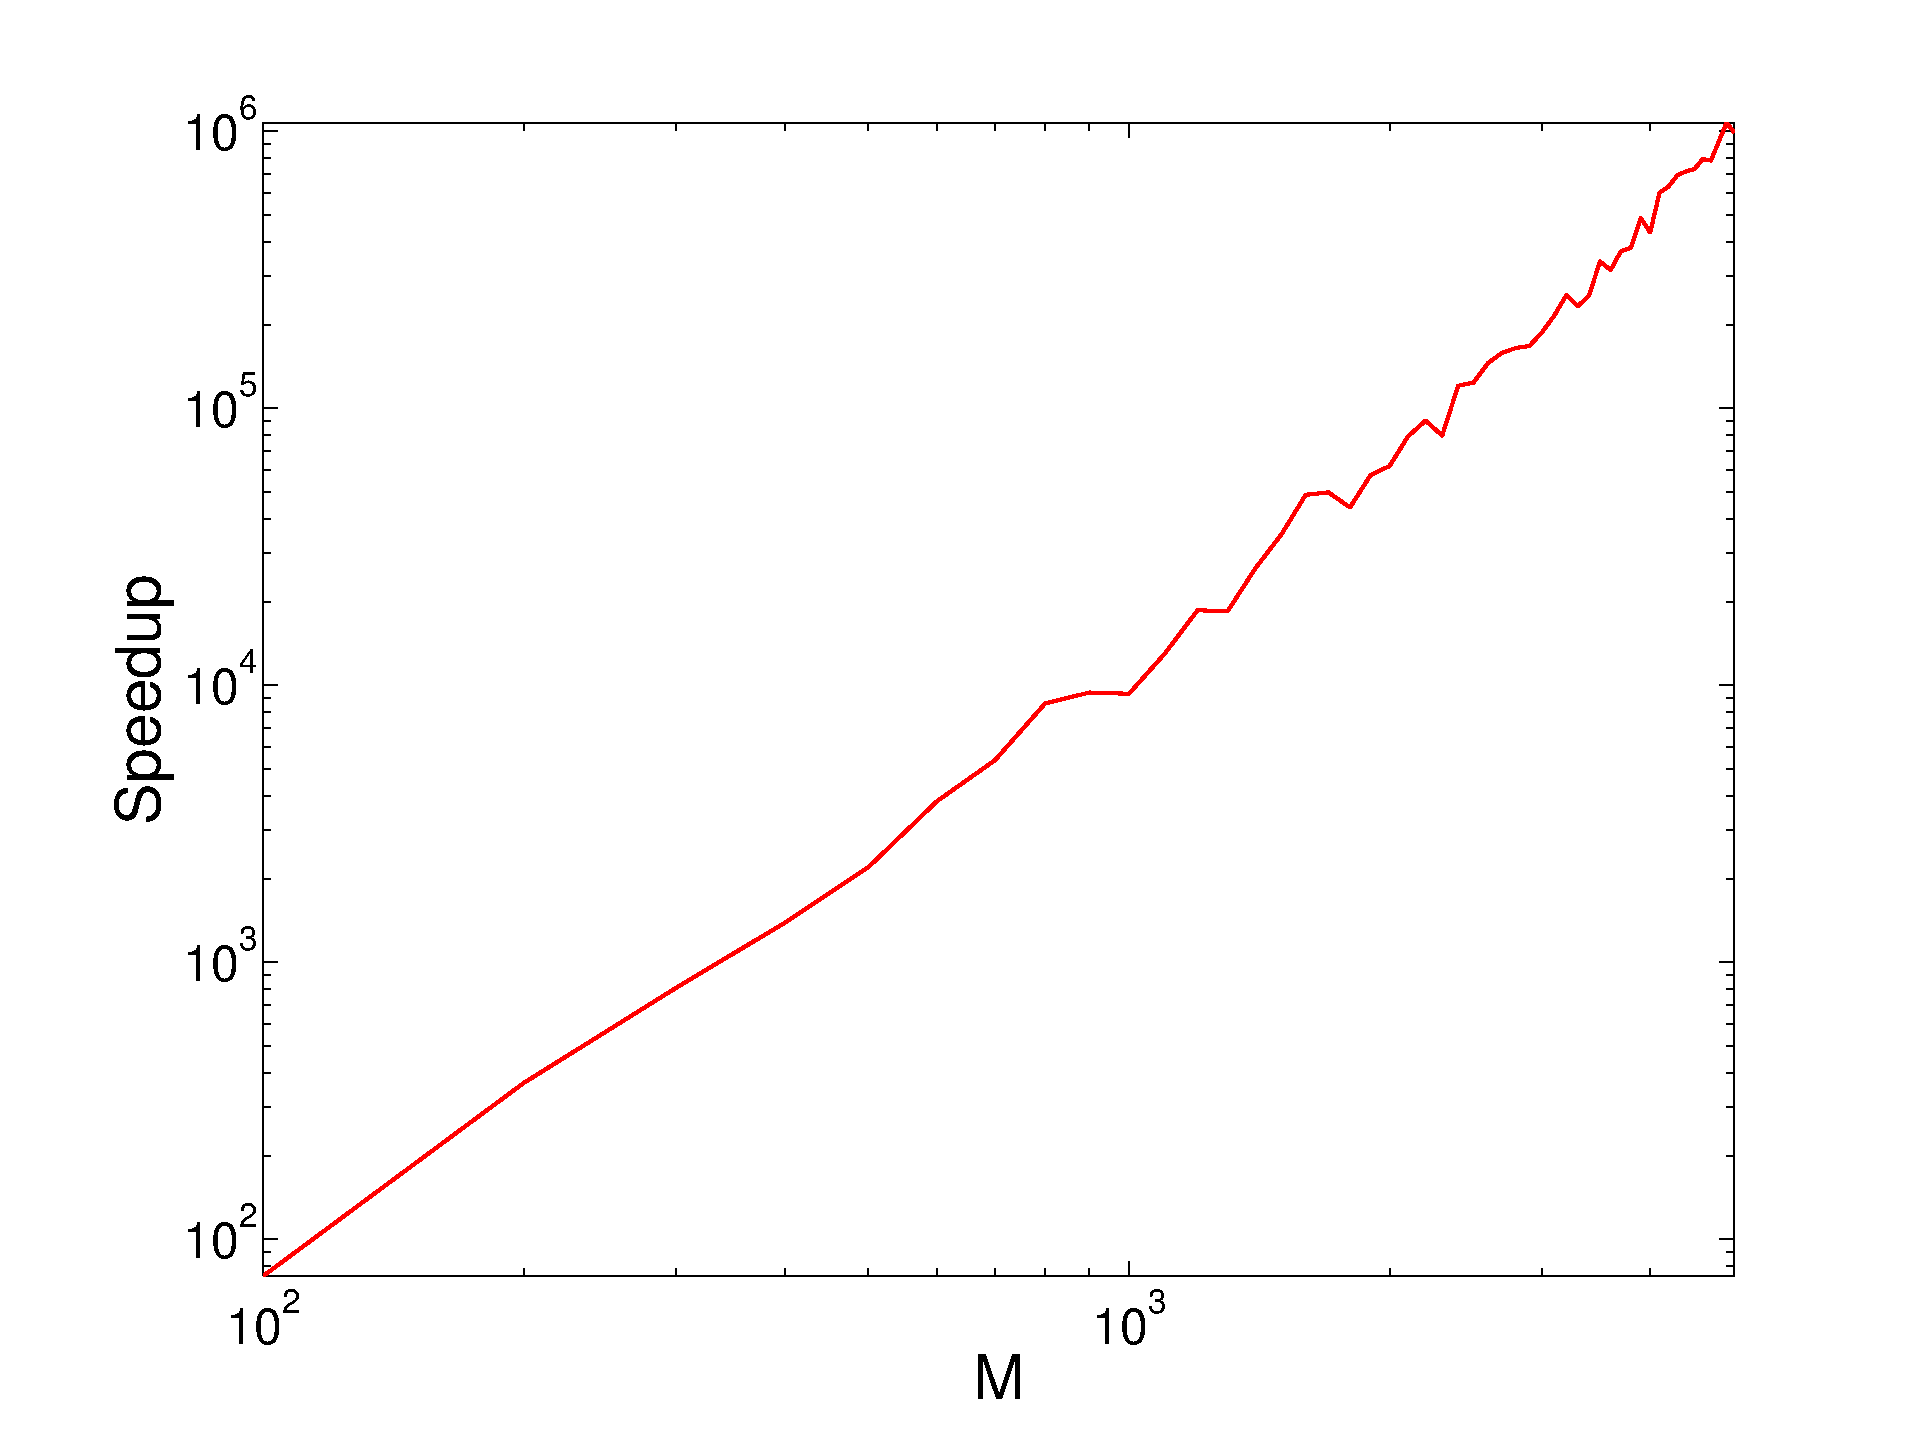
\includegraphics[width=0.5\textwidth,height=0.35\textwidth]{figMInvSpeedUp.eps}
  \caption{Speedup of ODC framework prediction on either TGP or GPR while retrieving precomputed matrix inverses as $M$ increases, compared with computing them on test time by KNN scheme (log-log scale)}
  \label{fig:SpeedUp}
\end{figure}
Having accomplished the performance analysis which comprehensively interprets our parameters, we used the recommended setting to compare the performance with other methods and show the benefits of this framework. Figure~\ref{fig:SpeedUp}\ignore{start by showing} shows the speedup gained by retrieving the matrix inverses on test time, compared with computing them at test time by NN scheme. The figure shows significant speedup from precomputing local kernel machines.  
%\vspace{-1.5mm}

Table~\ref{tab:tblRes} shows error, training time and prediction time of NN, FIC, and different variations of ODC  on Poser and Human-Eva datasets. Training time is formatted as ($t_c$ + $t_p$),  where $t_c$ is the clustering time and $t_p$ is the remaining training time excluding  clustering.  As indicated in the top part of table ~\ref{tab:tblRes}, TGP  under our ODC-framwork can significantly speedup the prediction compared with NN-scheme in ~\cite{Bo:2010}, while achieving competitive performance; better in case Poser Dataset. As illustrated in our analysis in Figure~\ref{fig:ODCAnalysis}, higher overlap ($p$) gives better performance. From time analysis perspective, higher $p$ costs more training time due that more subdomains are created and trained.  While, Figure~\ref{fig:ODCAnalysis} and Table~\ref{tab:tblRes} indicates that AB-Ekmeans gives better performance than RPC under both GPR and TGP, AB-Ekmeans takes more time for clustering. Yet,  it is feasible to compute in all the datasets, we used in our experiments. Our experiments also indicate that as $p \to 1$ in TGP and GPR,    $K'=2$ and $K'=3$ takes double and triple the prediction time respectively, compared with $K'=1$, with almost no error reduction\ignore{; see detailed table in the SM}. We also compared our model to FIC in case of GPR, and our model achieved smaller error and smaller prediction time; see bottom part in Table~\ref{tab:tblRes}. However, TGP consistently gives better results on both Poser and HumanEva datasets. We also tried full TGP and GPR on Poser and Human Eva Datasets. Full TGP error is $5.35$ for Poser and $40.3$ for Human Eva. Full GPR error is $6.10$ for Poser and $59.62$ for Human Eva. The results indicate that ODC achieves either better or competitive to the full models. Meanwhie, the speedup is sigbificant for TGP prediction ($21X$ for Human Eva and $11X$  for Poser Datasets); see Fig.~\ref{fig_TGP_speedup_hp}. For GPR prediction, we achieved the best performance and the lowest prediction time compared to existing GPR prediction methods; see Fig.~\ref{fig_GPR_speedup_hp}.

Based on our comprehensive experiments on HumanEva and Poser datasets, we conducted an experiment on Human3.6M  dataset with TGP kernel machine, where $M = 1390$, $t=1$,  $p = 0.6, K'=1$, Ekmeans for clustering. We achieved a speedup of ${41.7X}$ on prediction time using our ODC framework  compared with NN-scheme, i.e., $7$ days if NN-scheme is used versus $4.03$ hours in our case with our MATLAB implementation. The error is $13.5$ (cm) for NN and $13.8$ (cm) for ODC; see Fig.~\ref{fig_TGP_speedup_h36}.

\begin{figure}
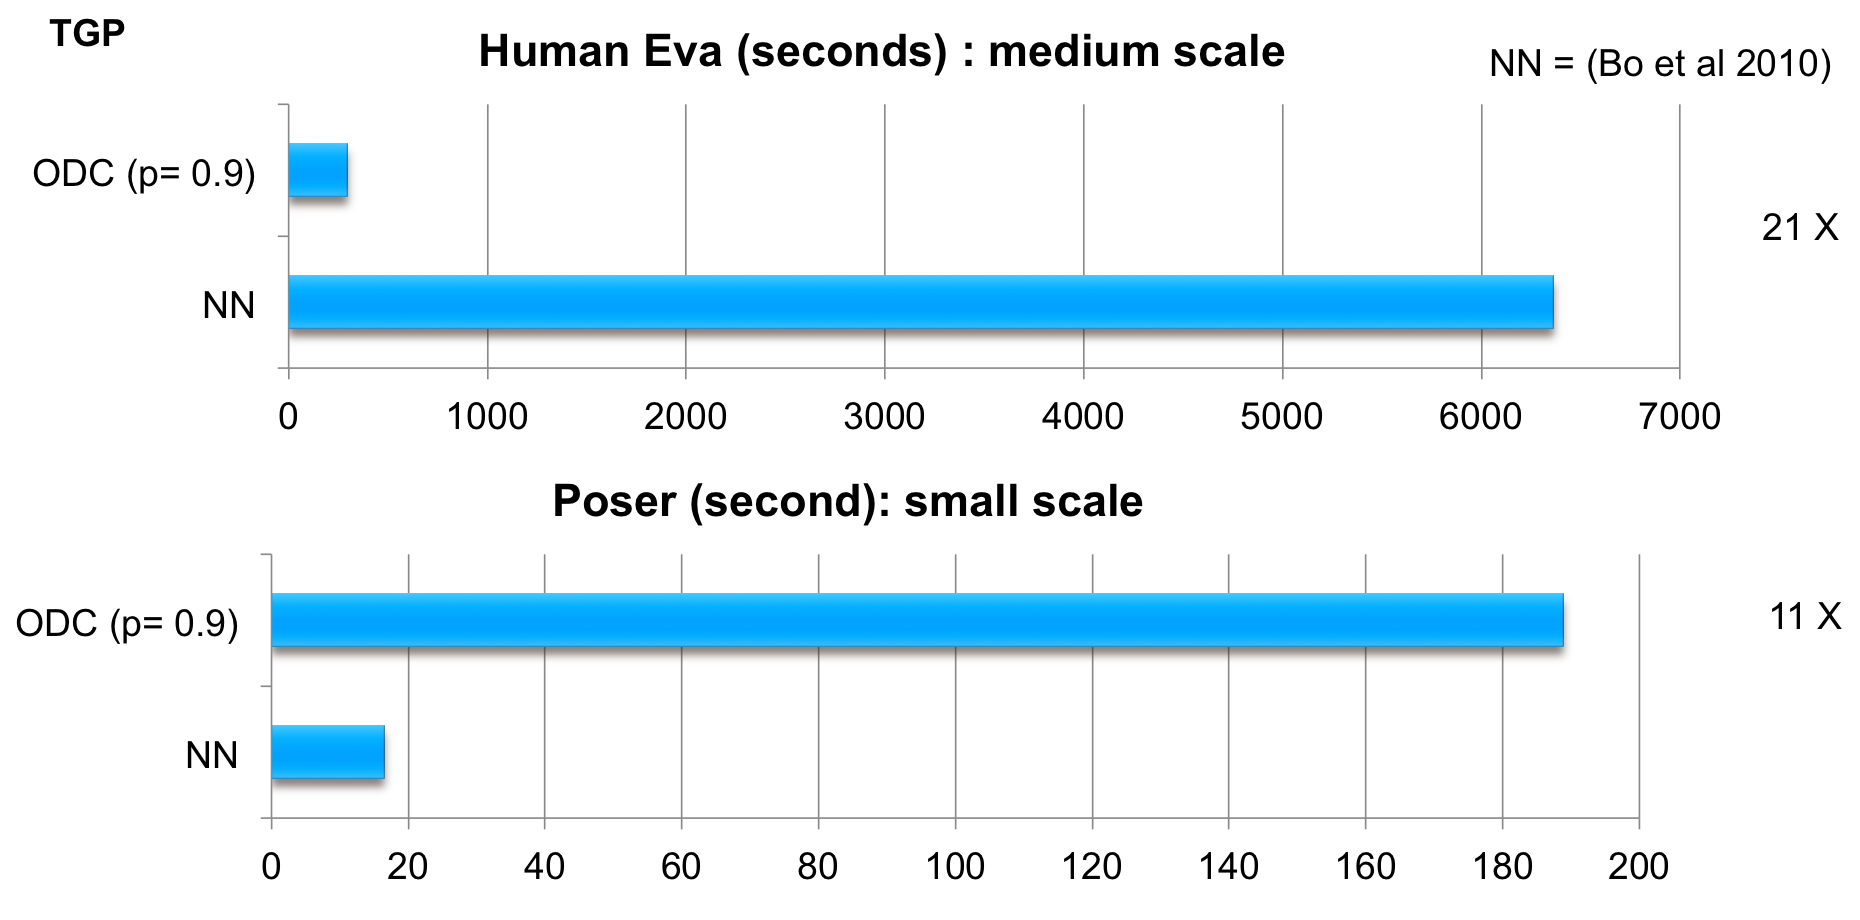
\includegraphics[width=0.5\textwidth]{TGP_speed_HEva_Poser.png}
\caption{TGP Human Eva Dataset (Speed)}
\label{fig_TGP_speedup_hp}
\end{figure}


\begin{figure}
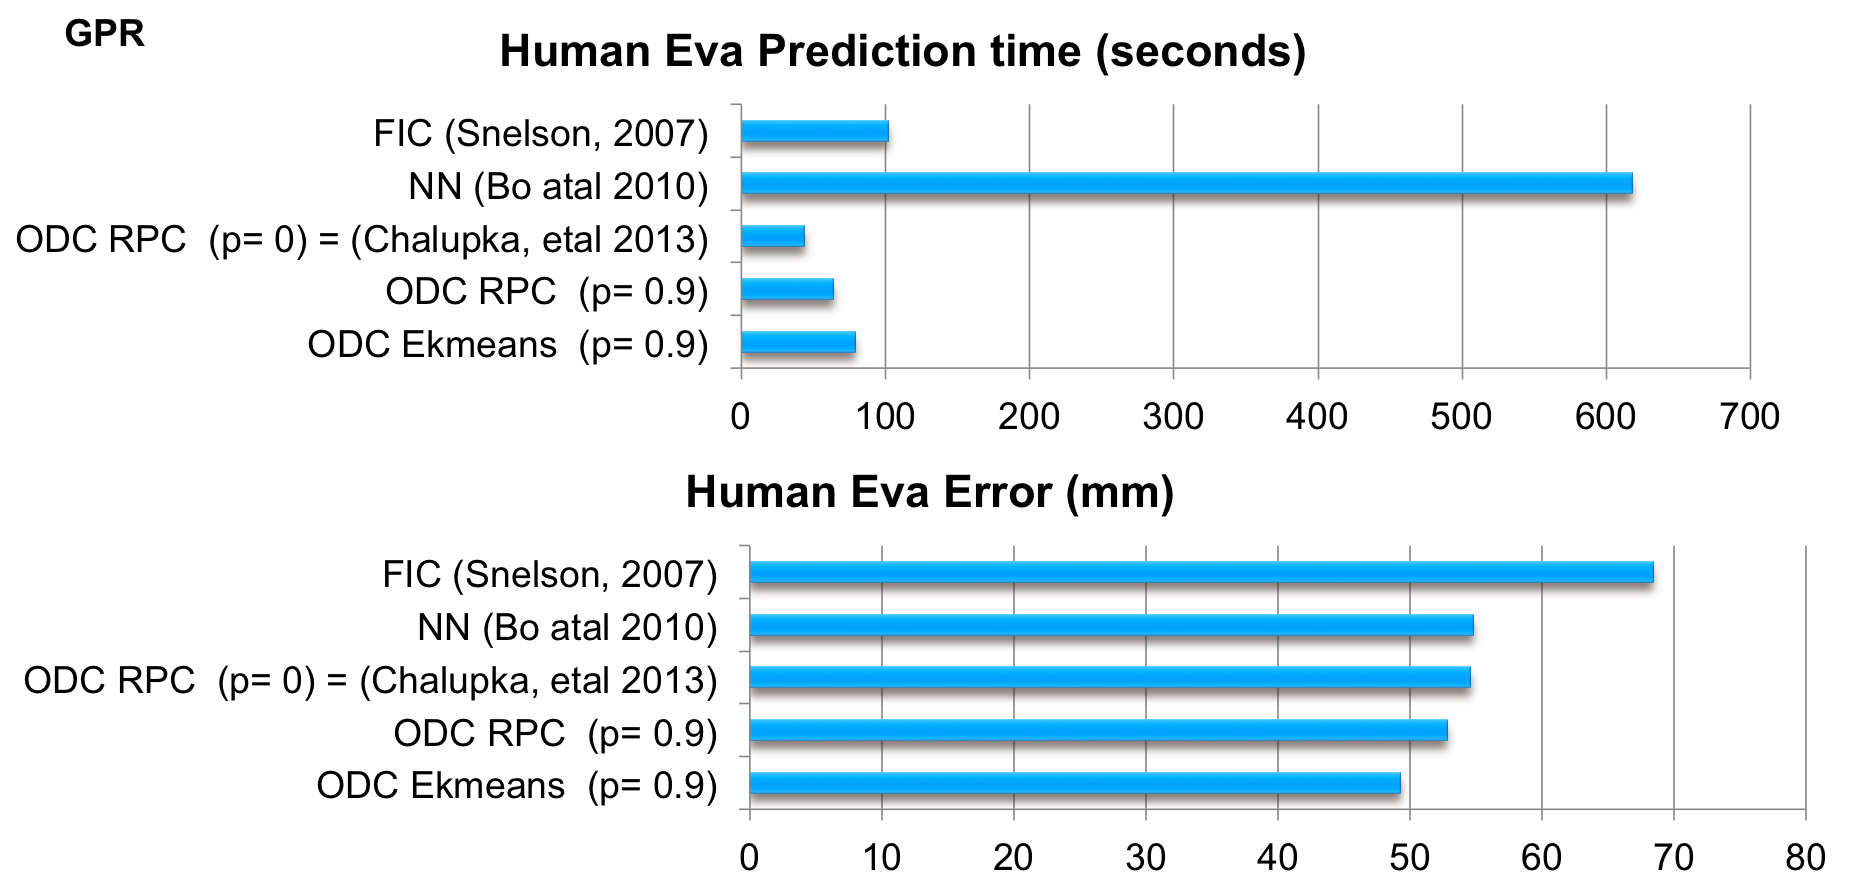
\includegraphics[width=0.5\textwidth]{GPR_speed_error_HumanEva.png}
\caption{GPR speed and error (Human Eva Dataset)}
\label{fig_GPR_speedup_hp}
\end{figure}


\begin{figure}
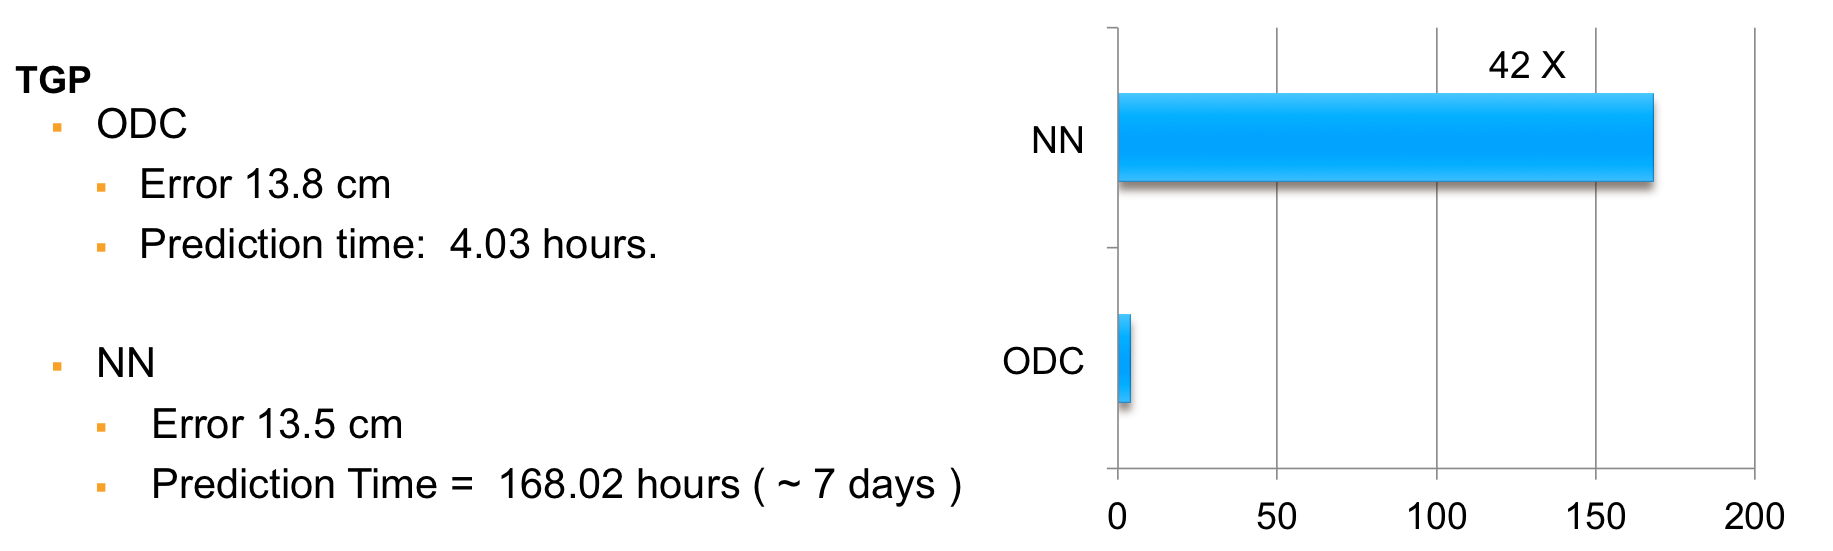
\includegraphics[width=0.5\textwidth]{TGP_speed_error_Human36.png}
\caption{TGP speed and error (Human3.6M Dataset)}
\label{fig_TGP_speedup_h36}
\end{figure}




\ignore{
We compare the performance of the proposed methods TGP-ODC and IWTGP-ODC against TGP-KNN \cite{Bo:2010} and IWTGP-KNN \cite{Yamada:2012}, respectively. We report performance on three publicly available datasets: Poser \cite{Trig06}, HumanEva \cite{SigalBB10} and Human3.6M \cite{human3m}. 
\begin{table}[htbp!]
  \centering
      \vspace{4pt}
  \caption{Error and Time for Poser and Human Eva datasets (on 2.6GHZ intel core i7), M = 800}
    \vspace{3pt}
    \scalebox{0.5}{
    \begin{tabular}{|l|l|lll|lll|}%ccc}
    \toprule
          &   & \textbf{Poser} & \textbf{} &       & \textbf{HumanEva} &       &      \\% & \textbf{Human 3.6} &       &  \\
    \midrule
         & & \textbf{Error (deg)} & \textbf{Training Time} & \textbf{Prediction Time} & \textbf{Error (mm) } & \textbf{Training Time} & \textbf{Prediction Time} \\%& \textbf{Error} & \textbf{Training Time} & \textbf{Prediction Time} \\
 \textbf{TGP}   & \textbf{NN} & 5.43       &  -     &    188.99 sec   & \textbf{38.1}      &  -     & 6363.823 sec \\%       &       &       &  \\
  & \textbf{ODC ($p= 0.9, t=1, K'=1$)-Ekmeans} & \textbf{5.4 }     &      (3.7 +25.1 ) sec  &   \textbf{16.5}  sec  &    \textbf{38.99 }  &  (2001 + 45.4) sec    &  \textbf{298.4} sec\\%       &       &       &  \\
    & \textbf{ODC ($p= 0.9, t=1, K'=2$)-Ekmeans} & {5.53}     &      (3.7 +29.46 ) sec  &   47.04  sec  &    {39.2 }  &  (2001 + 45.24) sec    &  569.6946  sec\\%       &       &       &  \\
      & \textbf{ODC ($p= 0.9, t=1, K'=3$)-Ekmeans} & {5.4}     &      (3.7 +28.8 ) sec  &   71.4 sec  &    {40.9 }  &  (2001 +  45.7) sec    &  721.0 sec\\%       &       &       &  \\
    & \textbf{ODC ($p= 0, t=1, K'=1$)-Ekmeans} &   7.6    &    (3.9 + 1.33) sec   &   14.8 sec  &    41.87   & (240 + 4.9832 ) sec       &  256.7709 \\%      &       &       &  \\
       & \textbf{ODC ($p= 0, t=1, K'=2$)-Ekmeans} &   12.3    &    (3.9 + 2.69) sec   &   42.25 sec  &    136.52 & (240 + 4.7790  ) sec       &  514.93 \\%      &       &       &  \\
       & \textbf{ODC ($p= 0, t=1, K'=3$)-Ekmeans} &   12.52    &    (3.9 + 1.86) sec   &    72.38 sec  &    187.72   & (240 + 4.7547 ) sec       &  770.9781 \\%      &       &       &  \\
      &  \textbf{ODC ($p= 0.9, t=1, K'=1$)-RPC} & 5.6      &      (0.23 +41.6 ) sec  &   15.8 sec  &   39.9  &    ( 0.45 + 49.05) sec     & 277.25 sec\\%       &       &       &  \\
         &  \textbf{ODC ($p= 0.9, t=1, K'=2$)-RPC} & 5.52      &      (0.23 +43.80 ) sec  &   43.802 sec  &   40.41  &    ( 0.45 + 46.77) sec     & 677.52 sec\\%       &       &       &  \\
        &  \textbf{ODC ($p= 0.9, t=1, K'=3$)-RPC} & 5.59  &      (0.23 +43.05 ) sec  &   67.11 sec  &    41.21&    ( 0.45 + 47.63) sec     &  882.6725 sec\\%       &       &       &  \\
  &  \textbf{ODC ($p= 0, t=1, K'=1$)-RPC} &   7.7    &   (0.15 + 1.717) sec   &   13.89 sec  &  42.32    &  (0.19 + 5.2551)      sec &  241.64 sec\\%      &       &       &  \\
    &  \textbf{ODC ($p= 0, t=1, K'=2$)-RPC} &   9.29 &   (0.15 + 1.83) sec   &   41.86 sec  &  58.99    &  (0.19 + 5.16)      sec &  475.14 sec\\%      &       &       &  \\
      &  \textbf{ODC ($p= 0, t=1, K'=3$)-RPC} &   12.47    &   (0.15 + 1.80) sec   &   66.42 sec  &  136.49    &  (0.19 + 5.20)      sec &  721.49 sec\\%      &       &       &  \\
      \hline
  \textbf{GPR}  & \textbf{NN} & 6.77      &   -    &  24 sec     &   54.8    &      - &    617.8  sec \\%&       &       &  \\
   & \textbf{ODC ($p= 0.9, t=1 , K'=1$)-Ekmeans} &  \textbf{6.27}      &  (3.7 +11.1 ) sec  &       \textbf{0.56}  sec & \textbf{49.3}  &   (2001 + 42.85)sec & \textbf{78.85} sec \\%       &       &       &  \\
   & \textbf{ODC($p= 0.0, t=1 , K'=1$)-Ekmeans} & 7.54      &   ( 3.9 + 1.38 sec) &    0.35 sec   & 49.6  &  (240 + 6.4) sec  &  48.1 sec\\%      &       &       &  \\
  & \textbf{ODC ($p= 0.9, t=1 , K'=1$)-RPC} &  6.45      &  (0.23 +17.3 ) sec  &       0.52  sec & 52.8  & (0.49 + 46.06) sec     &  64.13 sec\\%       &       &       &  \\
    & \textbf{ODC ($p= 0.0, t=1 , K'=1$)-RPC  = ~\cite{Chalupka:2013}} &   7.46    &   (0.15 + 1.47) sec &    0.27 sec   & 54.6  &  (0.261 + 4.58 ) sec & 43.52 sec\\%      &       &       &  \\
    & \textbf{FIC ~\cite{fic06}} &   7.63 (+/- 0.4)  &   (- + 20.63)   &    0.3106     &   68.36(+/- 0.84)    &  -     & 101.5442 (+/- 1.36) sec\\%      &       &       &  \\
    \bottomrule
    \end{tabular}}%
  \label{tab:tblRes}%
\end{table}%
}
%\textbf{ODC-Parameters}
% Table generated by Excel2LaTeX from sheet 'Sheet1'

%\input{experimentssubold}